\clearpage
\section{Sharing data - Publication of two complex electrophysiological datasets}
\label{sec:data}

Scientific progress is a sequence of scientific findings building on top of each other. These findings are classically hypothesis tested against experimental data and the resulting interpretation is communicated to other scientists via the publication of a manuscript. In recent years, however, the practice of publishing papers has been criticized for a lack of robustness. Attempts in a number of scientific fields, including among others life sciences, to reproduce published scientific findings failed to support the same conclusions \citep{Baker_2016, Fidler_2017, Pashler_2012, Ioannidis_2005, Goodman_2007, Ioannidis_2007, OpenScienceCollaboration_2015}. To qualitatively distinguish between different levels of reproducibility, a collection of terms has been applied: reproducibility, replicability, repeatability \citep{Plesser_2018, Drummond_2009}. However the specific interpretation of each of these terms highly depends on the scientific field they are applied in. Repeatability for example can be the re-performance of the same experimental study using identical components. However, for computer sciences repeating an experiment might be the re-running of the same software simulation on the same machine using the same software packages. Replicating a study by running the same code on the identical machine might be a realistic project, whereas running the identical experiment in psychology is not \citep{Anderson_2016}. A widely accepted version of reproducibility terminology by \citet{Goodman_2007} is therefore omitting the terms 'replicability' and 'repeatability' for simplification and defines instead three different types of reproducibility \citep[from][]{Plesser_2018}:

\begin{description}
 \item[Methods reproducibility] \hfill \\ \textit{'provide sufficient detail about procedures and data so that the same procedures could be exactly repeated.'}
\item[Results reproducibility] \hfill \\ \textit{'obtain the same results from an independent study with procedures as closely matched to the original study as possible.'}
\item[Inferential reproducibility] \hfill \\ \textit{'draw the same conclusions from either an independent replication of a study or a reanalysis of the original study.'}
\end{description}


This definition of 'methods reproducibility' highlights another important aspect of scientific publications: the underlying data. Reproducing findings of publications is harder for older publications \citep{Vines_2013}, which to a large part can be accounted for by the decreasing retrievability of the original datasets. The obligation to provide research data to other scientists is a standard introduced already decades ago by many funding initiatives (e.g. NIH since 2003\footnote{\url{https://grants.nih.gov/grants/policy/data_sharing/}} \todo{mention nfdi here?}) for publications in a number of journals (e.g. Springer Nature\footnote{\url{https://www.springernature.com/gp/authors/research-data-policy/data-availability-statements/12330880}}), however the readiness to comply is rather low (1/10 publications provides research data on request \citep{Savage_2009}). To address the problem of reproducibility for original research articles, a number of journals were opened, which invite to publish replications of the original articles in computational science \footnote{ReScience, \url{http://rescience.github.io/}}, economics\footnote{\url{http://www.economics-ejournal.org/special-areas/replications-1}}, psychology\footnote{\url{https://www.apa.org/pubs/journals/xge/replication-articles}} and neuroscience \citep{Yeung_2017}.

To improve the situation of data availability, \citet{Wilkinson_2016} defined the Fair Principles, providing guidelines to make research data Findable, Accessible, Interoperable, Reusable. Complementing these guidelines, a number of sites have become available for hosting scientific data (Zenodo\footnote{Zenodo, \url{https://zenodo.org/}}, Pangaea\footnote{Pangaea, \url{https://www.pangaea.de}}, BMC Research Notes\footnote{BMC Research Notes, \url{https://bmcresnotes.biomedcentral.com/} \& \url{https://bmcresnotes.biomedcentral.com/about/introducing-data-notes}}, DataDryad\footnote{Datadryad, \url{https://datadryad.org/}}, GIN\footnote{GIN, \url{https://gin.g-node.org/}},EuDat\footnote{EuDat, \url{https://eudat.eu/}} Research Data Australia\footnote{RDA, \url{https://www.ands.org.au/online-services/research-data-australia/rda-registry}}, \citep{Assante_2016}) and publishing data descriptor papers (ScientificData\footnote{ScientificData, \url{https://www.nature.com/sdata/}}, DataScience\footnote{DataScience, \url{https://datascience.codata.org/}} \citep{Candela_2015}).
It has been shown, that mandated data archiving upon publication highly improves data availability \citep{Vines_2013}. Going one step further, \citet{Chen_2019} show that making only the data available is not sufficient for reproducible science, data need to be accompanied by software packages used for further analysis. In the optimal case this encompasses detailed analysis motivation a complete analysis workflow. Making the effort of publishing the data is possible for large scale datasets, e.g. from particle physics \citep{Jomhari_2017}.

In this section, we provide an example of two complex published datasets from the neuroscientific field \citep{Brochier_2018}, demonstrating the size of data and metadata involved in such an experiment and the amount of data preparation needed for analysis and publication. We present the pipeline used for metadata aggregation and discuss its strengths and shortcomings. Parts of the pipeline are published in \cite{Zehl_2016} where they serve as example cases for metadata handling practices.


% replication, reproducibility - different field different meaning
% 
% Scientific data as basis for findings
% Current system: experiment - analysis - paper -> manuscript publication
% Reprodicibility crisis in science
% 
% Different levels of reproducibility: reusablility, replicability, reproducibility... and the interpretation depends on the scientific field
% 
% first problem: data sharing, second problem: code and workflow sharing
% reasons for this: 'ownership of data, human data' additional effort of preparation not included in funding
% 
% immediate approach for past research: reproduction papers: ReScience,...
% solultions for 1): fair principles, data publications (add list of journals, repositories for hosting)
% solutions for 2) partially also addressed by data journals [open data is not enough]


% \todo{replication, reproducibility - different field different meaning https://www.nature.com/articles/s41567-018-0342-2}
% \todo{fair principles}
% 
% Reproducibility of scientific results is a recently highly debated topic.
% Making research data available for the scientific community is 
% 
% \todo{ReScience}
% 
% \todo{Data hosting sites: https://www.pangaea.de/submit/ https://bmcresnotes.biomedcentral.com/about/introducing-data-notes}
% \todo{Horizon 2020 - Open Access as a standard way of publishing  - text as well as research data %https://www.bmbf.de/upload_filestore/pub/Open_Access_in_Deutschland.pdf
% }
% 
% \todo{The Availability of Research Data Declines Rapidly with Article Age https://www.cell.com/current-biology/fulltext/S0960-9822(13)01400-0}
% 
% \todo{open data is not enough - include analysis and metadata -  CERN Analysis Preservation and REANA https://www.nature.com/articles/s41567-018-0342-2}
% \todo{Reuse of large data possible - CMS example (The CERN Open Data port) http://opendata.cern.ch/record/5500}



% Abstract We publish two electrophysiological datasets recorded in motor cortex of two macaque monkeys during an instructed delayed reach-to-grasp task, using chronically implanted 10-by-10 Utah electrode arrays. We provide a) raw neural signals (sampled at 30kHz), b) time stamps and spike waveforms of offline sorted single and multi units (93/156 SUA and 49/19 MUA for monkey L and N, respectively), c) trial events and the monkey's behavior, and d) extensive metadata hierarchically structured via the odML metadata framework (including quality assessment post-processing steps, such as trial rejections). The dataset of one monkey contains a simultaneously saved record of the local field potential (LFP) sampled at 1kHz. To load the datasets in Python, we provide code based on the Neo data framework that produces a data structure which is annotated with relevant metadata. We complement this loading routine with an example code demonstrating how to access the data objects (e.g., raw signals) contained in such structures. For Matlab users, we provide the annotated data structures as mat-files.
% 

% \subsection{Publication of two complex electrophysiological datasets}
In \citet{Brochier_2018} we publish two complete high-dimensional electrophysiological datasets containing Utah Array recordings from monkey motor cortex. Recording subjects are two macaque monkeys (monkey L and N) which performed a complex instructed delayed reach-to-grasp task. Each recording contains continuously sampled data from 96 electrodes accompanied by the corresponding spiking activity. Spikes were extracted during online recording and offline sorted using the \software{Plexon Offline Sorter}\footnote{Plexon Offline Sorter, \url{https://plexon.com/products/offline-sorter/}}. Electrophysiological data are accompanied by a number of behavioral and control signals. Detailed metadata were aggregated and are provided in the \software{odML} format (see \cref{sec:scidata_metadata_structure,sec:metadata}).

\rewrite{Complex datasets, as the two provided here (high-dimensional, multi-scale during complex behavior), are a challenge for performing reproducible analysis. Besides the often rather variable nature of the circumstances under which such data were recorded, the data additionally experience a number of often interactively performed preprocessing steps before they can be used in actual data analyses. Without a detailed knowledge about all these steps, the actual data analysis may be biased or strongly affected. In most cases, electrophysiological data available as open source are in this respect not sufficiently annotated and documented. For this reason, we provide here a comprehensive description of how and under which circumstances the datasets were recorded as well as a detailed description of preprocessing steps that need to be considered before performing analyses on the data. We additionally publish a machine-readable format of these metadata including our parameters and results of the described preprocessing steps. We are aware that all this information may not be sufficient for the reproducible analysis of such data. The reason is that reproducible workflows including the provenance trail are not yet established for electrophysiological neuroscience, especially not for such complex experiments as presented here.}

\subsection{Relevance to the field}
The published datasets contain unique recordings from a complex electrophysiological setup. There are very few datasets of this type of experiment with this level of complexity available, wherefore we provide a valuable addition to the openly available dataset collection. The datasets are interesting for multiple reasons and can be used in a variety of contexts:
\begin{itemize}
 \item Public datasets are great for teaching and demonstration purposes. Especially for teaching it is important to not only work with toy examples, but having real-world data at hand. This improves the teaching quality and provides a better insight into the field.
 \item For analysis of coordinated population activity of neurons in the form of the local field (LFP) potential \citep{Mitzdorf_1985, Logothetis_2004, Einevoll_2013}. This datasets provides the opportunity to study LFP activity exhibiting wave activity across a spatially extended volume of cortex\citep{Denker_2018}.
 \item The datasets contain spiking activity from ~100 neurons recorded simultaneously. This permits analysis of spiking activity coordination, e.g. via correlation analysis \citep{Torre_2016, Torre_2016a, Quaglio_2017, Quaglio_2018}
 \item The availability of LFP as well as spiking data invites to study the relation between the two modalities, e.g. by relating synchrony in spiking activity to beta band power in the LFP \citep{Denker_2011}.
 \item Additionally to spiking and LFP data the dataset is also rich in behavioural aspects, since the monkey is performing a complex reach-to-grasp task involving two cues and a delay period. These datasets provide the opportunity to relate the previously described neuronal analysis to the behaviour of the animal.
 \item Based on the recording modalities described above, new methods for the analysis of spiking, LFP and behavioral data can be developed. This is of high interest since the number of electrodes recorded simultaneously increases drastically due to recent advances in electrode manufacturing and current analysis methods are at their capacities with current datasets \citep{Seo_2015,Jun_2017}. To be able to analyze neural data of the next generation, new approaches are needed. Potential candidates to deal with the problem of combinatorial explosion are dimensionality reduction methods like Gaussian-Process Factor Analysis (GPFA) \citep{Yu_2009}. 
 \item The published datasets together with the detailed description of metadata sources can serve as a starting point for development of a comprehensive metadata tracking system for neuroscientific experiments. Parts of this development are presented in later sections of this manuscript.
 \item The the correct identification of spikes based on a continuous recording trace (spike sorting) is a field of active research \citep{Rey_2015, Lefebvre_2016, Sukiban_2019}. For the evaluation of spike sorting algorithms, the availability of testing data is a critical. With this dataset we provide raw recording traces, automatically extracted threshold crossing events as well as a manual spike sorting to compare new spike sorting algorithms to.
\end{itemize}


% \subsubsection{Recording Modalities}
% The modalities recorded in the two example datasets can be separated in 3 categories: neuronal, behavioural \& control signals and metadata. The neuronal signals encompass continously sampled raw data, which are hardware filtered between band-pass filtered to $0.3Hz - 7.5kHz$


% \todo{describe continously sampled data in more detail, differences between monkeys, large number of simultaneously recorded single neurons (93 and 156, for L and N respectively) along with the continuous neuronal “raw” signals (sampled at 30kHz, and broadly band-pass filtered to 0.3Hz - 7.5kHz)}


\todo{provide introduction to odml here or forward reference the odMLtables chapter? -> give detailed intro to odml here, since this is rather short in the odmltables chapter}
\subsection{The experiment}

The experiment is a complex reach-to-grasp task performed by macaque monkeys. The basic component of the experiment are displayed in \cref{fig:r2g_introduction}. The two monkeys are trained to attend two cues coding for the grip type and force to perform. After the second cue the monkey performs the movement, pull the object and holds it to receive a reward. At the same time neuronal activity is recorded from motor and premotor areas of the cortex via a chronically implanted Utah Array. 

The subjects of the experiment are two Rhesus macaque monkeys (Macaca mulatta) who were trained to perform the delayed reach-to-grasp task prior to implantation of the recording arrays. Details on the two subjects are summarized in \ref{tab:scidata_data_overview}. Depending on the monkey character and learning abilities the different instruction steps (accustoming to the experimenter, setup, different versions of the task) requires multiple months of daily training. The training was completed when the monkey had an average success rate of 85\% of the trials in the standard task setting.
The two monkeys trained for the task differ in gender, active hand of the task and character resulting in different behaviours observed during the recording task. As monkey N is rather calm and less motivated he is in general performing shorter sessions and less trials per session as monkey L, who is eager to work (see \cref{tab:scidata_data_overview}). A recording day typically consisted of multiple recording sessions, whereas each session lasts between $10$ and $20$ minutes resulting in an average working time per weekday of $1.5$ hours. Weekends and holidays were usually excluded from training and recording.


\begin{figure}[!ht]
\begin{center}
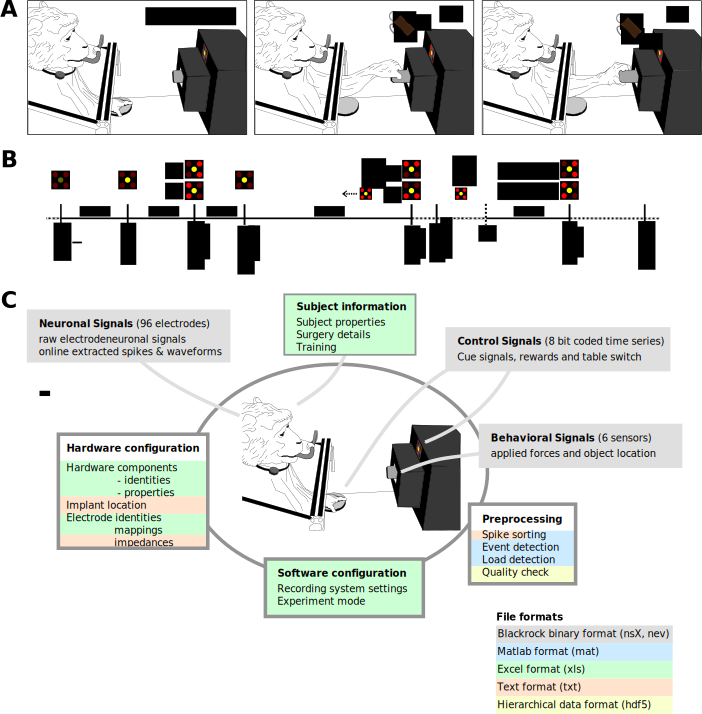
\includegraphics[width=\textwidth]{figures/scidata_experiment}
\caption[Components of the Reach-to-Grasp experiment]{Components of the Reach-to-Grasp experiment. A) The monkey is located in a monkey chair, his active hand resting the home position (left panel). The monkey performs an instructed, delayed reach towards an object. Two grip conditions (side grip/precision grip (SG/PG, respectively)) can be instructed via visual cues. B) Visual cues are presented via five LEDs located at the height of the monkeys eyes. The monkey initialized a trial by holding the home switch with his active hand for $400$ milliseconds, then the central LED is activated and stays active for the complete trial. Two complementary cues are presented with a delay of $1000$ milliseconds, coding for the grip type and the force needed to move the object. The of the four corner LEDs, always two neighboring ones are activated. The two vertical arrangements code for the grip type and the horizontal ones for the force type. After the second cue (GO-ON), the monkey releases the home switch (SR-ON), reaches for the object (hold start, HS) and holds it for $500$ milliseconds. Then a reward is delivered and the monkey can initiate the next trial by returning to the resting configuration and holding the home switch again. C) The data acquired during a recording session comprise neural activity signals, as well as behavioral and control signals. Metadata is captured in multiple formats, encompassing hard- and software components and settings as well as information about the subject and post-processing steps performed on the the data. Figure modified from \citet{Brochier_2018}.}
\label{fig:r2g_introduction}
\end{center}
\end{figure}

\begin{table}[]
\scriptsize
\begin{tabular}{|l|l|l|l|l|l|l|l|}
\hline
                                                                                              & \multicolumn{3}{l|}{\textbf{monkey L}}                                                                   & \multicolumn{3}{l|}{\textbf{monkey N}}                                                            & \textbf{description}                                                                             \\ \hline
\multicolumn{8}{|l|}{\textbf{Monkey}}                                                                                                                                                                                                                                                                                                                                                                           \\ \hline
gender                                                                                        & \multicolumn{3}{l|}{female}                                                                              & \multicolumn{3}{l|}{male}                                                                         &                                                                                                  \\ \hline
birthdate                                                                                     & \multicolumn{3}{l|}{15th March 2004}                                                                     & \multicolumn{3}{l|}{15th May 2008}                                                                &                                                                                                  \\ \hline
weight                                                                                        & \multicolumn{3}{l|}{5kg}                                                                                 & \multicolumn{3}{l|}{7kg}                                                                          &                                                                                                  \\ \hline
active hand                                                                                   & \multicolumn{3}{l|}{left}                                                                                & \multicolumn{3}{l|}{right}                                                                        &                                                                                                  \\ \hline
character                                                                                     & \multicolumn{3}{l|}{\begin{tabular}[c]{@{}l@{}}eager to work\\ quick\\ efficient\\ nervous\end{tabular}} & \multicolumn{3}{l|}{\begin{tabular}[c]{@{}l@{}}slow learner\\ calm\\ less motivated\end{tabular}} &                                                                                                  \\ \hline
Utah array rotation                                                                           & \multicolumn{3}{l|}{216$^\circ$}                                                                          & \multicolumn{3}{l|}{239$^\circ$}                                                                   &                                                                                                  \\ \hline
\textbf{Recording}                                                                            &                                        &                                &                                &                                      &                              &                             &                                                                                                  \\ \hline
session name (*)                                                                              & \multicolumn{3}{l|}{\textbf{l101210-001}}                                                                & \multicolumn{3}{l|}{\textbf{i140703-001}}                                                         &                                                                                                  \\ \hline
session files                                                                                 & *.ccf                                  & \multicolumn{2}{l|}{108.2 kB}                                   & *.ccf                                & \multicolumn{2}{l|}{187.1 kB}                              & cerebus configuration                                                                            \\ \hline
                                                                                              & *.nev                                  & \multicolumn{2}{l|}{287.7 MB}                                   & .nev                                 & \multicolumn{2}{l|}{168.3 MB}                              & \begin{tabular}[c]{@{}l@{}}digital events\\ unsorted spikes times\\ spike waveforms\end{tabular} \\ \hline
                                                                                              & *-02.nev                               & \multicolumn{2}{l|}{287.7 MB}                                   & *-03.nev                             & \multicolumn{2}{l|}{168.3 MB}                              & \begin{tabular}[c]{@{}l@{}}digital events\\ sorted spikes times\\ spike waveforms\end{tabular}   \\ \hline
                                                                                              & *.ns2                                  & \multicolumn{2}{l|}{8.5 MB}                                     & *.ns2                                & \multicolumn{2}{l|}{204.7 MB}                              & \begin{tabular}[c]{@{}l@{}}analog signals of object sensors\\ LFP (only monkey N)\end{tabular}   \\ \hline
                                                                                              & *.ns5                                  & \multicolumn{2}{l|}{4.1 GB}                                     & *.ns6                                & \multicolumn{2}{l|}{5.8 GB}                                & raw neuronal signal                                                                              \\ \hline
                                                                                              & *.odml                                 & \multicolumn{2}{l|}{2.7 MB}                                     & *.odml                               & \multicolumn{2}{l|}{2.3 MB}                                & metadata                                                                                         \\ \hline
recording start                                                                               & \multicolumn{3}{l|}{Fr, 10th Dec 2010 10:50am}                                                           & \multicolumn{3}{l|}{Th, 3rd Jul 2014 10:41am}                                                     &                                                                                                  \\ \hline
recording duration                                                                            & \multicolumn{3}{l|}{11:49 min}                                                                           & \multicolumn{3}{l|}{16:43 min}                                                                    &                                                                                                  \\ \hline
daily recording id                                                                            & \multicolumn{3}{l|}{1}                                                                                   & \multicolumn{3}{l|}{1}                                                                            &                                                                                                  \\ \hline
\begin{tabular}[c]{@{}l@{}}number of recordings\\ same day\end{tabular}                       & \multicolumn{3}{l|}{9}                                                                                   & \multicolumn{3}{l|}{3}                                                                            &                                                                                                  \\ \hline
\begin{tabular}[c]{@{}l@{}}total daily \\ recording time\end{tabular}                         & \multicolumn{3}{l|}{01:28 h}                                                                             & \multicolumn{3}{l|}{00:51 h}                                                                      &                                                                                                  \\ \hline
\multicolumn{8}{|l|}{\textbf{Performance}}                                                                                                                                                                                                                                                                                                                                                                      \\ \hline
\begin{tabular}[c]{@{}l@{}}recorded trials\\ (total/error/\\ grip error/correct)\end{tabular} & \multicolumn{3}{l|}{204}                                                                                 & \multicolumn{3}{l|}{160}                                                                          &                                                                                                  \\ \hline
\begin{tabular}[c]{@{}l@{}}trials performance\\  correct/error (grip error)\end{tabular}      & 135                                    & \multicolumn{2}{l|}{69 (12)}                                    & 135                                  & \multicolumn{2}{l|}{19 (16)}                               &                                                                                                  \\ \hline
\begin{tabular}[c]{@{}l@{}}trial types\\  SG-LF/SG-HF\end{tabular}                            & 41                                     & \multicolumn{2}{l|}{30}                                         & 35                                   & \multicolumn{2}{l|}{35}                                    &                                                                                                  \\ \hline
\begin{tabular}[c]{@{}l@{}}trial types\\  PG-LF/PG-HF\end{tabular}                            & 31                                     & \multicolumn{2}{l|}{33}                                         & 35                                   & \multicolumn{2}{l|}{36}                                    &                                                                                                  \\ \hline
\multicolumn{8}{|l|}{\textbf{Spikesorting}}                                                                                                                                                                                                                                                                                                                                                                     \\ \hline
\# SUA                                                                                        & \multicolumn{3}{l|}{93}                                                                                  & \multicolumn{4}{l|}{156}                                                                                                                                                                             \\ \hline
\# MUA                                                                                        & \multicolumn{3}{l|}{49}                                                                                  & \multicolumn{4}{l|}{19}                                                                                                                                                                              \\ \hline
\# electrodes with SUA                                                                        & \multicolumn{3}{l|}{65}                                                                                  & \multicolumn{4}{l|}{78}                                                                                                                                                                              \\ \hline
\begin{tabular}[c]{@{}l@{}}\# electrodes with \\     SUA or MUA\end{tabular}                  & \multicolumn{3}{l|}{86}                                                                                  & \multicolumn{4}{l|}{89}                                                                                                                                                                              \\ \hline
\end{tabular}
\caption[Overview of subjects and recording sessions]{Overview of monkeys, recording session files and dates, spike sorting and monkey performance. The monkeys differ in gender, age, weight and active hand used for the task. Information is provided about individual recording files, sessions, performance of the monkey as well as single unit (SUA) and multi unit activity (MUA). \todo{add more descriptions in table and nicefy table}}
\label{tab:scidata_data_overview}
\end{table}


For recording of neural activity, each monkey had a single Utah array\footnote{Blackrock Microsystems, Salt Lake City, UT, USA} implanted in the motor cortex contralateral to the active hand. The Utah array is an electrode array with 100 electrodes arranged in a $10\times10$ grid. 96 of 100 of the iridium coated electrodes can be used for recording (\cref{fig:implant_locations}). The individual electrodes are $1.5mm$ long, $400\mu m$ apart and have an average pre-implantation impedance of $50k\Omega$. The electrode array is connected to a head stage via a fiber bundle connecting individual electrodes to contact of the CerePort Connector, which is a connector external to the skin permitting the daily coupling of the implant to the recording setup. In addition to the array electrodes one ground and two reference electrodes are implanted. During the implantation surgery the skull was opened and the dura removed to pneumatically insert the Utah array into the cortex. The dura and skull were close, whereby the cables were arranged to lead to the connector which was attached to the skull on the other hemisphere. The Utah arrays were implanted a few millimeters anterior to the central sulcus and they were rotated before implantation to cover the arm/hand representation of the primary motor cortex as well as parts of premotor cortex (\cref{fig:implant_locations}).

The task the monkeys had to perform involved grasping an object using one of two grip types: side (SG) or precision grip (PG). Detailed sketches of the different grips are depicted in\cref{fig:r2g_introduction} A center and top panel. For both grip types the position of thumb (T), index (I) and middle (M) finger are indicated relative to the profile of the object. The force required to pull the object towards the monkey was either about $1N$ (low force) or $2N$ (high force).  In a trial the monkey was always instructed by the first cue a(CUE) bout the grip type (SG/PG) and with the second cue (GO) about the force level (LF/HF), resulting in 4 different trial types (SGLF, SGHF, PGLF, PGHF) possible. The first and second cue are presented with $1s$ delay in which the monkey has to memorize the presented grip type and can prepare for the movement, which can be initialized after the second (GO) cue. Cues are presented by combinations of two of five illuminated LEDs. The encoding of the grip and force type can be seen in \cref{fig:r2g_introduction} B (CUE-ON and GO-ON). The setup consisted of three main parts, the neural recording platform for acquisition of neuronal signals, the experimental apparatus providing the environment for performing the task and the behavioral control system controlling and coordinating the task procedure (\cref{fig:scidata_setup_overview}).

\paragraph{Differences between the datasets}
In principle the same setup was used for both monkeys, however small deviations exist which are highlighted in the corresponding figures in yellow (monkey L) and red (monkey N). The four main aspects area
\begin{description}
 \item[Recording Arrays] the recording from different Utah arrays, including different electrode mapping as well as a different implant location
 \item[Connecting Hardware] Usage of different hardware for connecting the implant with the data acquisition system. The two headstages (samtec/patient cable) influence the recording quality by their specific electrical properties.
 \item[Software versions and settings] The recording software versions and setting differ, since an update was available between the recordings. This includes the usage of different file extensions for recordings of continuous data (ns5 in monkey L vs ns6 in monkey N) and additionally a downsampled and filtered version of the neural data being recorded in the ns2 format for monkey N. Furthermore the number of samples extracted online for each of the threshold crossing events was extended from 39 samples in monkey L to 48 samples in monkey N.
 \item[Experiment Control] The LabView program controlling and monitoring the task was updated which leads to the usage of different binary coding for digital events (\cref{tab:bit_translation}). 
\end{description}


\begin{figure}
 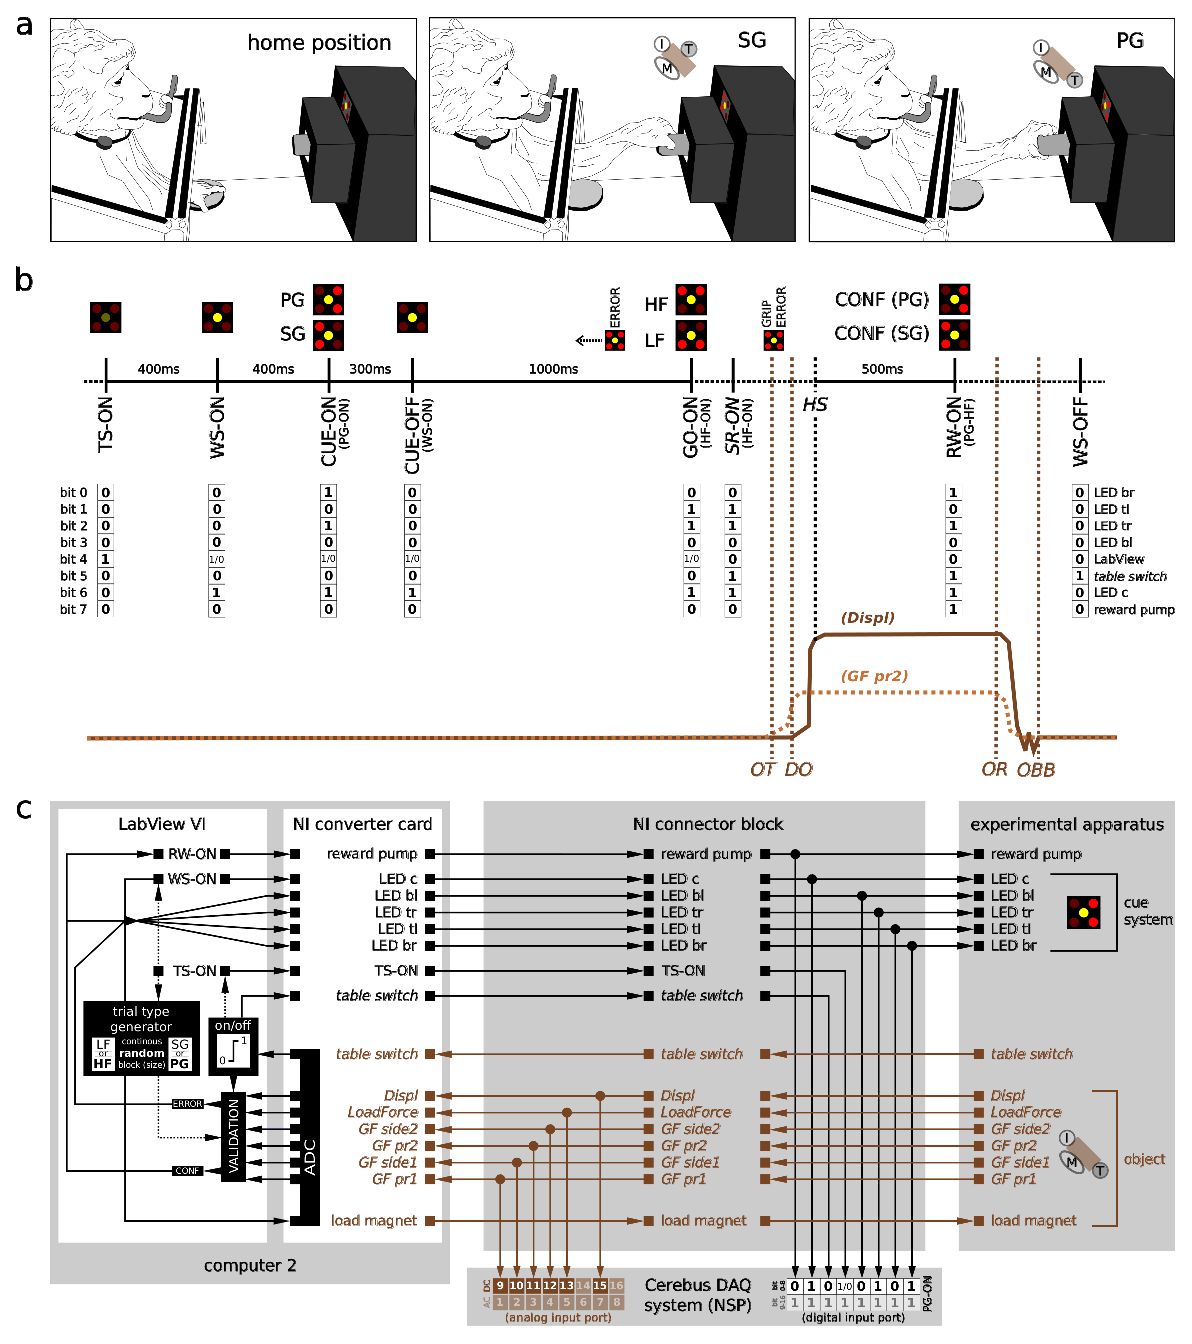
\includegraphics[width=0.7\textwidth]{./figures/scidata_figures/task_trialscheme}
 \caption[Overview of the experimental apparatus and behavioral control system.]{\rewrite{Overview of the experimental apparatus and behavioral control system. (a) Sketches of the experimental apparatus and the monkey performing the reach-to-grasp task. Left: monkey in its home position with the working hand on the table switch. Middle and right: monkey grasping the object with a side grip (SG) and a precision grip (PG), respectively. Insets of middle and right sketch show the actual position of the index finger (I), the thumb (T), and the middle finger (M) on the object (brown cube) 11 . (b) Trial scheme of an example trial with
the respective visual cues (different illumination combinations of the 5 LEDs illustrated on top) shown to the monkey at its respective times. The behavioral events are marked along the time axis (see main text for abbreviations). Events with black font mark digitally recorded events, whereas events with brown font indicate events (object touch OT, object release OR, displacement onset DO, and object back to baseline OBB) which were extracted offline from baseline deviations of the analog signals of the object’s sensors. Additionally, we indicate by italic fonts events which were generated by the monkey, while all other events are produced by LabView. The 8-bit binary code for the digital event signals sent from LabView VI to the NSP at the respective times is shown below the time axis. Example traces for the analog signals of the HE sensor (Displ; dark solid line) and one of the 4 FSR sensors located at the object’s surface (GF pr2, light dotted line) used to monitor the monkeys behavior and extract
OT, OR, DO, and OBB are shown at the bottom. (c) Outline of the devices and their wiring controlling the behavior. All analog signal streams are colored in brown, whereas all digital signal streams are colored in black.} Figure from \cite{Brochier_2018}.}
\label{fig:task_trialscheme}
\end{figure}

\begin{figure}
 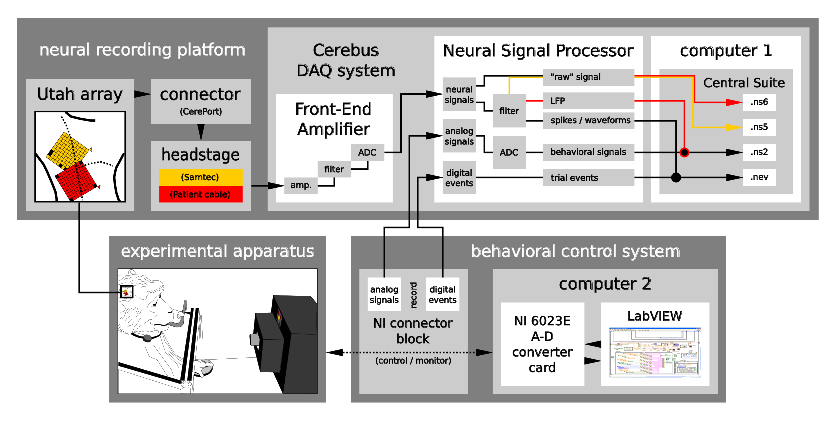
\includegraphics[width=\textwidth]{./figures/scidata_figures/setup_overview}
 \caption[Overview of the setup]{\rewrite{Overview of the setup. The setup consisted of three main parts: the neural recording platform, the experimental apparatus, and the behavioral control system. The neural recording platform (top) was composed of the implanted Utah array with its corresponding connector (CerePort), a headstage (Samtec or Patient cable), and the Cerebus data acquisition (DAQ) system (i.e. the Front-End Amplifier, Neural Signal Processor (NSP), and the Cerebus control software, Central Suite, installed on the setup computer 1). The experimental apparatus (bottom left) consisted of the physical devices which the monkeys had to interact with (i.e., the visual cue panel (square with 5 LEDs), the target object, the table switch, and the reward system). The behavioral control system (bottom right) was built from hard- and software of National Instruments (NI, National Instruments Corporation, Austin, Texas, USA). It was composed of a NI connector block which was linked via a NI 6023E A-D converter card to setup computer 2 on which the NI system design software, LabView, was running. To record the behavioral data the behavioral control system was interlinked with the neuronal recording platform via the NSP and the NI connector block. All three parts are separately described in more detail in the main text, as well as Figures 2 and 4. Setup differences between the two monkeys are indicated in yellow and red for monkeys L and N, respectively.} Figure from \cite{Brochier_2018}.}
 \label{fig:scidata_setup_overview}
\end{figure}

\begin{table}[]
\footnotesize
\begin{tabular}{|l|l|l|l|l|l|}
\hline
sensor & channel ID & label     & located at       & activated by          & used to identify  \\ \hline
FSR 1  & 137        & GF pr1    & object’s top     & index finger’s touch  & PG type           \\ \hline
FSR 2  & 138        & GF side1  & object’s left    & middle finger’s touch & SG type           \\ \hline
FSR 3  & 139        & GF pr2    & object’s bottom  & thumb touch           & PG type           \\ \hline
FSR 4  & 140        & GF side2  & object’s right   & thumb touch           & SG type           \\ \hline
FSR 5  & 141        & LoadForce & object’s spring  & object loading        & pulling force     \\ \hline
HE     & 143        & Displ     & object's shuttle & object displacement   & object’s position \\ \hline
\end{tabular}
 \caption[Overview of six objects sensonsr to monitor and control the monkey's behavior]{\rewrite{Overview of the six object sensors used to monitor and control the monkey's behavior. The first four force sensitive resistance (FSR) sensors are used to monitor the applied grip type. They are located on the surface of each object side and are activated by the touch of the corresponding monkey's finger. The fifth FSR is located at the spring counterbalancing the pull resistance of the object and is used to measure the pulling force applied by the monkey. The hall-effect sensor (HE) is located along the low-friction shuttle of the object and used to measure the position of the object. The signals of all sensors are saved in the ns2 with the stated channel ID and label (cf. \cref{fig:cerebus_system}).} Table from \cite{Brochier_2018}.}
 \label{tab:overview_sensors}
\end{table}

\begin{table}[]
\scriptsize
\begin{tabular}{|l|l|l|l|l|l|l|l|l|l|c|l|}
\hline
\textbf{\begin{tabular}[c]{@{}l@{}}decimal\\ code\end{tabular}} & \multicolumn{8}{c|}{\textbf{(8-bit) binary code}}                                                                                                                                                                           & \multicolumn{3}{c|}{\textbf{trial interpretation}}                                                 \\ \hline
                                                                & bit 7         & bit 6                           & bit 5           & bit 4       & bit 3                            & bit 2                            & bit 1                            & bit 0                            & \multicolumn{2}{l|}{}                                                                     & monkey \\ \hline
\textbf{65296}                                                  & 0             & 0                               & 0               & 1           & 0                                & 0                                & 0                                & 0                                & \multicolumn{2}{l|}{\textbf{TS-ON}}                                                       & L,N    \\ \hline
\textbf{65280}                                                  & 0             & 0                               & 0               & 0           & 0                                & 0                                & 0                                & 0                                & \multicolumn{2}{l|}{\textbf{TS-OFF}}                                                      & L      \\ \hline
\textbf{65344}                                                  & 0             & 1                               & 0               & 0           & 0                                & 0                                & 0                                & 0                                & \multicolumn{2}{c|}{\multirow{2}{*}{\textbf{WS-ON}}}                                      & L      \\ \cline{1-9} \cline{12-12} 
\textbf{65360}                                                  & 0             & 1                               & 0               & 1           & 0                                & 0                                & 0                                & 0                                & \multicolumn{2}{c|}{}                                                                     & N      \\ \hline
\textbf{65360}                                                  & 0             & 1                               & 0               & 1           & 0                                & 0                                & 0                                & 0                                & \multirow{2}{*}{\textbf{PG-ON}}                      & \multirow{4}{*}{\textbf{(CUE-ON)}} & L      \\ \cline{1-9} \cline{12-12} 
\textbf{65365}                                                  & 0             & 1                               & 0               & 1           & 0                                & 1                                & 0                                & 1                                &                                                      &                                    & N      \\ \cline{1-10} \cline{12-12} 
\textbf{65354}                                                  & 0             & 1                               & 0               & 0           & 1                                & 0                                & 1                                & 0                                & \multirow{2}{*}{\textbf{SG-ON}}                      &                                    & L      \\ \cline{1-9} \cline{12-12} 
\textbf{65370}                                                  & 0             & 1                               & 0               & 1           & 1                                & 0                                & 1                                & 0                                &                                                      &                                    & N      \\ \hline
\textbf{65344}                                                  & 0             & 1                               & 0               & 0           & 0                                & 0                                & 0                                & 0                                & \multicolumn{2}{l|}{\multirow{2}{*}{\textbf{CUE-OFF}}}                                    & L      \\ \cline{1-9} \cline{12-12} 
\textbf{65360}                                                  & 0             & 1                               &                 & 1           & 0                                & 0                                & 0                                & 0                                & \multicolumn{2}{l|}{}                                                                     & N      \\ \hline
\textbf{65353}                                                  & 0             & 1                               & 0               & 0           & 1                                & 0                                & 0                                & 1                                & \multirow{2}{*}{\textbf{LF-ON}}                      & \multirow{4}{*}{\textbf{(GO-ON)}}  & L      \\ \cline{1-9} \cline{12-12} 
\textbf{65369}                                                  & 0             & 1                               & 0               & 1           & 1                                & 0                                & 0                                & 1                                &                                                      &                                    & N      \\ \cline{1-10} \cline{12-12} 
\textbf{65350}                                                  & 0             & 1                               & 0               & 0           & 0                                & 1                                & 1                                & 0                                & \multirow{2}{*}{\textbf{HF-ON}}                      &                                    & L      \\ \cline{1-9} \cline{12-12} 
\textbf{65366}                                                  & 0             & 1                               & 0               & 1           & 0                                & 1                                & 1                                & 0                                &                                                      &                                    & N      \\ \hline
\textbf{65385}                                                  & 0             & 1                               & 1               & 0           & 1                                & 0                                & 0                                & 1                                & \multirow{2}{*}{\textbf{SR}}                         & \multicolumn{1}{l|}{(+LF)}         & L,N    \\ \cline{1-9} \cline{11-12} 
\textbf{65382}                                                  & 0             & 1                               & 1               & 0           & 0                                & 1                                & 1                                & 0                                &                                                      & \multicolumn{1}{l|}{(+HF)}         & L,N    \\ \hline
\textbf{65509}                                                  & 1             & 1                               & 1               & 0           & 0                                & 1                                & 0                                & 1                                & \multirow{2}{*}{\textbf{RW-ON}}                      & \multicolumn{1}{l|}{(+CONF-PG)}    & L,N    \\ \cline{1-9} \cline{11-12} 
\textbf{65514}                                                  & 1             & 1                               & 1               & 0           & 1                                & 0                                & 1                                & 0                                &                                                      & \multicolumn{1}{l|}{(+CONF-SG)}    & L,N    \\ \hline
\textbf{65376}                                                  & 0             & 1                               & 1               & 0           & 0                                & 0                                & 0                                & 0                                & \multicolumn{2}{l|}{\textbf{GO-OFF/RW-OFF}}                                               & L,N    \\ \hline
\textbf{65312}                                                  & 0             & 0                               & 1               & 0           & 0                                & 0                                & 0                                & 0                                & \multicolumn{2}{l|}{\multirow{2}{*}{\textbf{STOP}}}                                       & L,N    \\ \cline{1-9} \cline{12-12} 
\textbf{65280}                                                  & 0             & 0                               & 0               & 0           & 0                                & 0                                & 0                                & 0                                & \multicolumn{2}{l|}{}                                                                     & L      \\ \hline
\textbf{65391}                                                  & 0             & 1                               & 1               & 0           & 1                                & 1                                & 1                                & 1                                & \multicolumn{1}{c|}{\multirow{2}{*}{\textbf{ERROR}}} & \multirow{2}{*}{(+switch)}         & L      \\ \cline{1-9} \cline{12-12} 
\textbf{65359}                                                  & 0             & 1                               & 0               & 0           & 1                                & 1                                & 1                                & 1                                & \multicolumn{1}{c|}{}                                &                                    & L      \\ \hline
\multirow{2}{*}{}                                               & \textbf{pump} & \textbf{LED}                    & \textbf{switch} & \textbf{TS} & \multicolumn{4}{c|}{\textbf{LED}}                                                                                                         & \multicolumn{3}{l|}{\multirow{2}{*}{}}                                                             \\ \cline{2-9}
                                                                &               & \multicolumn{1}{c|}{\textbf{c}} & \multicolumn{2}{c|}{}         & \multicolumn{1}{c|}{\textbf{bl}} & \multicolumn{1}{c|}{\textbf{tr}} & \multicolumn{1}{c|}{\textbf{tl}} & \multicolumn{1}{c|}{\textbf{br}} & \multicolumn{3}{l|}{}                                                                              \\ \hline
\end{tabular}
\caption[Translation table of 8-bit binary to decimal event codes and their interpretation in a trial context]{\rewrite{Translation table of 8-bit binary to decimal event codes and their interpretation in a trial context. The 8-bit binary event code created by LabView states the activation (bit status 1) and deactivation (bit status 0) of the LEDs of the cue system (c:center, t:top, b:bottom, l:left, r:right), the table switch (switch), the reward pump (pump) or the trial start (TS) internally set by LabView. During each trial the (8-bit binary) status of these devices/settings (cf. bottom row) were sent from LabView to the NSP of the Cerebus DAQ system (Figure 2). There, the event codes were converted to a decimal code of the bit sequence assuming another byte with all bits set to 1 in front. The decimal event codes are found in the nev files with a time stamp. The correct interpretation of these events in context of a trial are here indicated in the second column from the right. Due to different versions of the LabView control program for monkey L and N the decimal codes for the same event may differ between the monkeys (cf. first column from the right). Some event codes (65381, 65386, 65390, 65440, 65504) are not listed here, because they do not have a concrete meaning and occur only sporadically in the nev file due to a mistake in the sampling of the digital events - they have to be ignored. Except for the "ERROR" codes, the event codes are sorted in sequential order from top to bottom with respect to the task, i.e. their order corresponds to the sequence found in the nev file in a reach-to-grasp trial. Note that some events are represented by the same decimal codes and are just differently interpreted due to their sequential occurrence in a trial (cf. TS-OFF and STOP, as well as WS-ON and CUE-OFF).} Table from \cite{Brochier_2018}.}
\label{tab:bit_translation}
\end{table}

\begin{figure}
 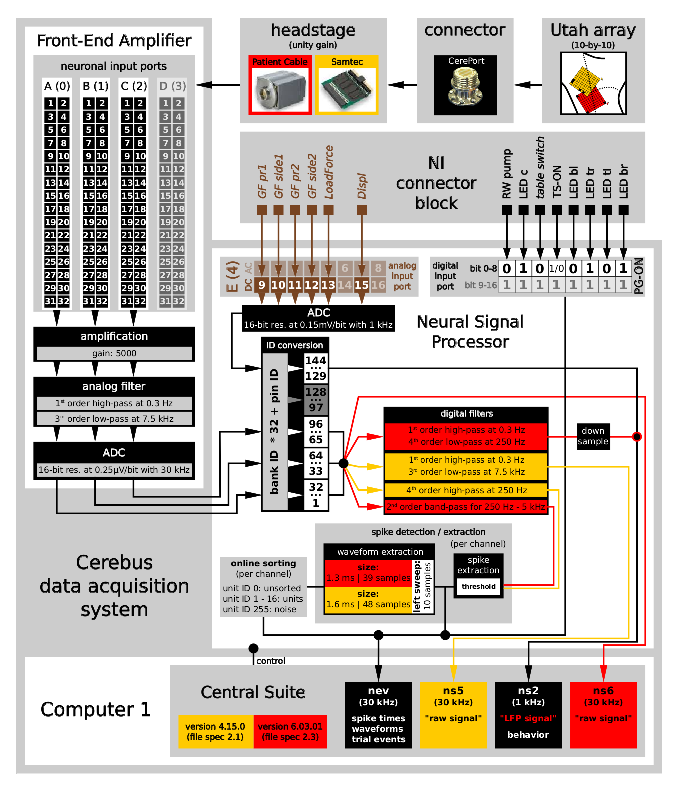
\includegraphics[width=0.7\textwidth]{./figures/scidata_figures/cerebus_system}
 \caption[Sketch of the components related to the recording of the neuronal signals]{\rewrite{Sketch of the components related to the recording of the neuronal signals. Data were recorded
using a Utah array, which was linked via its connector (CerePort) to a headstage (Samtec or Patient Cable) with a unity gain. From there the neural signals were transfered to the Cerebus Front-End Amplifier, where they were amplified, filtered and digitized. The digitized signals were converted into a single multiplex optical output and sent via a fiber-optic data link to the Neural Signal Processor (NSP), which is controlled by the Cerebus control software (Central Suite). Within the NSP the time points and waveforms of potential spikes were extracted online from a correspondingly processed copy of the neural signals and saved in the nev file. Simultaneously, the continuous raw signals (sampled at 30 kHz) were saved in the ns5 (for monkey L) or ns6 file (for monkey N). In parallel to the neural signals the NSP received also the digital trial events produced by the LabView VI, and the analog signals of the object’s sensors via the NI connector block of the behavioral control system. While the digital trial events were saved along with the extracted potential spikes in the nev file,
the analog signals of the sensors were digitized and saved in the ns2 file. For monkey N, a filtered and downsampled version of the neural signals (0.3–250 Hz at 1 kHz) was also saved in the ns2 file. Components and settings specific to monkey L and N are indicated by yellow and red, respectively.} Figure from \cite{Brochier_2018}.}
\label{fig:cerebus_system}
\end{figure}



\rewrite{

\subsection{Experimental apparatus}
\label{sec:experimental_apparatus}

The experimental apparatus was composed by a target object, a table switch, a visual cue, and a reward system. On each recording day, the monkey was seated in a custom-made primate chair and placed in front of that apparatus. The non-working arm of the monkey was loosely restrained in a semi-flexed position. To control the home position of the working hand between the reach-to-grasp movements, the table switch which was installed close to the monkey at waist level, 5cm lateral to the mid-line, needed to be pressed down. The target object was a stainless steel rectangular cuboid (40mm x 16mm x 10mm) rotated 45 degrees around the horizontal axis and pointing towards the monkey (\cref{fig:task_trialscheme}a). It was located 13cm away from the table switch at 14cm height. The posterior end of the object was attached through a low-friction horizontal shuttle to a counterweight hidden inside the apparatus, which was used to set the object load. The object load was set to one of two possible values to define the force type (LF and HF) needed for pulling the object in each trial by deactivating and activating an electromagnetic weight resting below the counterweight inside the apparatus. When activated, it attached to the counterweight and increased overall weight from usually 100gram to 200gram, which corresponds roughly to a pulling force of 1Newton and 2Newton for LF and HF, respectively. 

As already mentioned, the object was equipped with six sensors which monitored the monkey's reach-to-grasp behavior. Four force sensitive resistance sensors (FSR sensors) on the object surface provided continuous measurement of the grip forces applied on the object sides by the index and middle finger, as well as the thumb. The different activation patterns of these four FSR sensors, in particular the different placement of the thumb (see \cref{fig:task_trialscheme} a), were used to detect online if the correct grip type was performed. An additional FSR sensor was installed between the object and its counterweight. This FSR sensor was used to measure the horizontally applied force needed to oppose the corresponding object load. Due to the low, but still existing friction of the object moving inside the horizontal shuttle, the measured force signal of this sensor is not perfectly proportional to the horizontal force needed to lift the opposed object load, but sufficient to distinguish between LF and HF settings (cf., example in bottom right panel of \ref{fig:overview_data_l_1} and \ref{fig:overview_data_n_1}). The horizontal displacement of the object over a maximal distance of 15mm was measured by a hall-effect (HE) sensor. All sensors of the object are summarized in \cref{tab:overview_sensors}. The visual cue system, composed of a square of five LEDs (size 10 x 10 mm), was located just above the target object and used to instruct the monkey about the requested behavior. While the central yellow LED was used to warn the monkey that a trial had started, the four red corner LEDs were used to code separately the grip and the force type for the requested trial type of each trial. In this context the illumination of the two left, the two right, the two bottom, or the two top LEDs coded for SG, PG, LF, or HF, respectively (see \cref{fig:task_trialscheme} b for illustration). The reward system consisted of a bucket filled with apple sauce and equipped with a feeding tube and a pump allowing to deliver on demand the reward (few drops of the apple sauce) to the monkey (\cref{fig:task_trialscheme} a).

\subsubsection{Behavioral control system}
\label{sec:behavioral_control_system}

The core of the behavioral control system is a custom-made Virtual Instrument (VI) in LabView that controls the digital event sequence and the requested behavior of each trial in a recording. A digital event reflects hereby the activation or deactivation of a physical device of the experimental apparatus. In this context, the LabView VI is responsible to activate and deactivate the LEDs of the visual cue system, the reward pump, and the electromagnet. The latter is not controlled by a digital event, but by an analog square signal that switches the magnet on or off. To control the requested behavior, the LabView VI monitors the monkey's manipulation of the table switch and the target object. The table switch as well as all sensors of the target object produce continuous analog signals that are digitized by the NI converter card and fed into the LabView VI of the setup computer (see \cref{fig:scidata_setup_overview} computer 2). The square signal of the table switch is then online reinterpreted as digital activation or deactivation event. \cref{fig:task_trialscheme} c displays a schematic diagram on how the physical devices of the experimental apparatus are connected to the setup computer and controlled and monitored by the LabView VI. We will now describe a typical execution of the LabView VI during a recording session in more detail. 

The possible trial types were set to SG-LF, SG-HF, PG-LF, and PG-HF, alternating with equal probability randomly in sequence between trials. Once the settings of the overall task were defined, the LabView VI was started to repetitively run and control the event sequence and behavior for each trial during the recording session. 

Each single trial was run and controlled as follows: 

The LabView VI only started a trial when the monkey deactivated the table switch by pressing and holding it down (home position, \cref{fig:task_trialscheme} a, left). This required not much muscle activity, but simply the weight of the monkey's hand on top of the smooth-running switch. If the table switch was deactivated, the LabView VI internally initiated a trial with a short time delay (TS-ON). In parallel, the program picked randomly one of the possible trial types (e.g., SG-HF) and activated or deactivated the electromagnet accordingly to fit the chosen load force of the object (e.g., activated for HF). To inform (or warn) the monkey that a new trial has started, the central LED was illuminated 400ms after the trial was initiated by the program (WS-ON). Four hundred ms after WS-ON the grip type was revealed to the monkey by illuminating the corresponding corner LEDs of the chosen trial type (CUE-ON, e.g., left LEDs for SG-ON). The LEDs of this first cue were turned off again after 300ms (CUE-OFF). The CUE-OFF was followed by a 1000ms preparatory delay at the end of which the monkey was informed about the upcoming force type by again illuminating the corresponding corner LEDs of the chosen trial type (GO-ON, e.g., top LEDs for HF-ON). This second cue also served as a GO signal for the monkey to initiate the movement which was registered by the activation of the table switch (SR-ON) when the monkey released it after a variable reaction time (RT). The execution of the movement was composed of reaching, grasping, pulling and holding the object in the position window for 500ms. The LabView VI controlled the movement execution online by checking the used grip type, the object displacement and the hold time. For checking the grip type, the grasp of the object was registered by small deflections of the FSR surface sensor signals caused by the monkey's fingers. A FSR sensor was registered as activated if the deflection surpassed a predefined threshold. The pattern of activated FSR sensors was then used by the LabView VI to control if the monkey performed the requested grip type. This meant, in particular, to check for SG and PG, if the FSR sensor on the right (GF side2), or on the bottom (GF pr2) of the object was activated by the monkey's thumb, respectively (see \cref{fig:task_trialscheme} a, middle and right). The other 2 sensors that measured force from the index and middle fingers for the 2 grip types (GF side1, and GF pr1) were not controlled online. If the correct grip was detected, the grip cue was illuminated again as a positive feedback. To check the object displacement, the LabView VI measured if the deflection of the HE sensor signal of the object was within the two defined position thresholds (4 and 14mm). The time point at which the displacement signal surpassed the lower threshold was used by the LabView VI to define the estimated start of the holding period (HS) online. If the object remained within the position window for 500ms after the HS was set, LabView activated the reward pump which provided the monkey with a drop of apple sauce as reward for a successful trial. The time until the reward pump was deactivated again by LabView was proportional to the duration of the object hold in the position window, with a maximum duration and with this a maximum amount of reward for a 500ms holding period. With this mechanism, both monkeys rapidly learned to hold the object at least 500ms in nearly all trials. In parallel to the deactivation of the reward pump, LabView turned off all LEDs to indicate that the running trial ended (WS-OFF). The monkey was allowed to release the object at its own pace as soon as it received the reward. A new trial sequence was started by LabView (TS-ON) as soon as the monkey returned to the home position (new deactivation of the table switch).

An abort of the described trial sequence by LabView (error trial) was triggered by the following three scenarios: (i) the monkey released the table switch before the GO cue, (ii) the wrong grip type was registered, and (iii) the object was not pulled and held long enough in the position window. In case one of these scenarios were registered by LabView the trial was aborted. For monkey L, the LabView VI provided additionally a negative feedback when aborting a trial by flickering all LEDs three times. 

As displayed in \cref{fig:task_trialscheme} c. the behavioral control system was connected to the NSP of the Cerebus DAQ system to store the trial event sequence and the monkey's behavior of each trial in a recording along with the neural data registered by the neural recording platform. For this, the analog signals of the sensors of the target object were copied from the NI connector block to the analog input port of the Cerebus System NSP via DC coupled BNC cables and connectors. In the NSP they were digitized with a 16-bit resolution at 0.15 mV/bit and a sampling rate of 1kHz and saved in the ns2 file under the channel ids listed in \cref{tab:overview_sensors}. All digital or digitized events that register the activation and deactivation of the table switch, the LEDs of the cue system, and the reward pump, as well as the internally generated digital trial start event (TS-ON) were coded as a 8-bit binary signal (see \cref{tab:bit_translation}) and transferred via the NI connector block to a 16-bit DB-37 input port of the NSP where they occupy the first 8 digits (remaining digits are set to 1). In the NSP the now 16-bit binary signal of each event was stored in its decimal representation and with its corresponding time point in the nev file (see \cref{tab:bit_translation} and \cref{fig:cerebus_system}).


\subsubsection{Neural recording platform}
\label{sec:neural_recording_platform}
The recording of the neural signals was performed using a neural recording platform with components produced by Blackrock Microsystems (Salt Lake City, UT, USA, www.blackrockmicro.com). The platform consisted of the multi-electrode Utah array, a headstage, and a Cerebus data acquisition (DAQ) system. The latter is composed of a Front-End Amplifier, a real-time Neural Signal Processor (NSP) and the control software, Central Suite (version 4.15.0 and 6.03.01 for L and N, respectively), running on Windows XP for L, and Windows 7 for N on the setup computer 1 (see Fig. \cref{fig:cerebus_system}). The Cerebus DAQ system was also connected to the behavioral control system via the NI connector block to save the analog behavioral data and digital trial event signals that were described in the previous section in parallel with the neural signals. All data were transmitted from the NSP via an ethernet cable to be saved first locally on the setup computer 1. After a recording day, all recordings were transferred to a data server. In the following, we will describe the function of the different components of the neural recording platform in more detail.

The implant location of the Utah array, as well as the electrode configuration of the array of each monkey was described previously (see \cref{sec:surgery_array_location} and \cref{fig:implant_locations}). The electrode identification numbers (IDs) are determined by how the electrodes of the array are wired and connected to the Cerebus Front-End Amplifier. See \ref{sec:channel_ids} for details.

The analog Blackrock headstage with unity gain (Samtec for monkey L, and Patient Cable for monkey N) was used to reduce the environmental noise. Overall, the reduction of the noise was better with the Patient Cable than with the Samtec headstage.

In the Front-End Amplifier, each of the 96 neural signals was differentially amplified with respect to the reference input of its corresponding connector bank (gain 5000) and filtered with a 1st-order 0.3Hz high pass filter (full-bandwidth mode) and a 3rd-order 7.5kHz Butterworth low pass filter. After that, the band-pass filtered neuronal signals were digitized with a 16-bit resolution at 0.25V/bit and a sampling rate of 30kHz, in the following called “raw signal”. The digitized signals were converted into a single multiplexed optical output and transmitted via a fiber-optic data link to the NSP. In the NSP the raw signals were saved in a ns5-file for monkey L and in a ns6-file for monkey N. The file format depended on the firmware and software version of the Cerebus DAQ system. In addition to the neural signals, the NSP received the analog behavioral signal recorded by the behavioral control system via the analog input port. These behavioral signals were digitized and saved with a sampling rate of 1kHz in a ns2-file. For monkey N, the ns2-file also contained a filtered and downsampled version of the raw signals, in the following called “LFP data”. To extract the LFP data, a copy of the raw data was online digitally low-pass filtered at 250Hz (Butterworth, 4th order), and downsampled to 1kHz within the NSP.

The NSP performed also an online spike waveform detection and classification controlled via the Central Suite software. The sorted spikes were used for a first online inspection of the data as well as for selecting and saving the spike waveforms for offline sorting. For this purpose the neuronal raw signals were for monkey L online high-pass filtered at 250 Hz (Butterworth, 4th order) and for monkey N band-pass filtered between 250Hz and 5kHz (Butterworth, 2nd order). Afterwards, the waveforms were detected by threshold crossing (manually set). These waveforms were then sorted by requesting the signal from identified neurons to follow through up to five hoops set by the user (all individually for each channel). To get an overview of the quality of the data during the recordings, the sorted waveforms were displayed in the online classification window provided by Central Suite.

The thresholds (one for each channel) for the spike waveform detection were not modified during a session and were saved in the nev-file for each session along with all other settings (e.g. filter setting etc) and configurations of Central Suite. The data and corresponding settings of Central Suite can also be inspected offline using the Blackrock software CentralPlay even in the absence of the Blackrock hardware system. Each time the high-pass filtered signal passed the threshold, a snippet of 1.6ms (48 samples) for monkey L and 1.3ms (38 samples) for monkey N was cut and saved as potential spike waveform. The snippet was cut with 10 sample points before threshold crossing and 38 or 28 points after for monkey L or N, respectively. Waveforms identified as potential single units (online sorted spikes) were labeled with IDs from 1 to 16. Unsorted waveforms were labeled with ID 0. These potential spike waveforms were saved together with their respective time stamps in the nev-file. Due to the high number of electrodes, online spike-sorting was moderately reliable. We therefore decided to re-sort spiking activity offline on each channel using the Plexon Offline Spike Sorter (Plexon Inc, Dallas, Texas, USA, version 3.3, for details see \cref{sec:data_preprocessing}). Results of offline sorting were saved in a copy of the original nev-file with an updated file name. 

All data files (nev, ns5/6, ccf) were saved on disk and backed-up on a data server at the end of the recording sessions. The information collected here are partly taken from \citep{Riehle_2013, Zehl_2016}.


\subsubsection{Origin of the channel IDs}
\label{sec:channel_ids}

The neuronal signal inputs to the Front-End Amplifier were grouped into four banks (A-D or 0-3) from which only the first 3 were used. Each bank consists of a male header with 34 pins of which 32 were the neuronal signal input channels. The other two channels served as reference and ground, respectively. In Central Suite, the identification (ID) number of each electrode of the array is defined by the position on the input bank and pin of the Cerebus Front-End Amplifier. For this Central Suite multiplies the bank ID (0, 1, 2, or 3) with the number of pins for neural signal input channels (32) and adds the ID of the pin the electrode is connected to (cf. ID conversion in \cref{fig:cerebus_system}). The electrode wiring of the Utah array is, though, not coordinated to the input banks of the Front-End Amplifer which leads to spatially unordered electrode IDs. Nevertheless, Utah arrays are fabricated usually in the same way where the corner electrodes are unconnected leading to a default (unordered) electrode ID configuration (cf. electrode configuration of monkey N in \cref{fig:implant_locations}). If in the fabrication process one of the corner electrodes was registered to be of significantly higher quality than any other electrodes of the grid, the corner electrode was connected instead and thereby changed the corresponding electrode configuration (cf. electrode configuration of monkey L in \cref{fig:implant_locations}). This led to the different ID sequences of the arrays for monkey L and N (see \cref{fig:implant_locations}). To facilitate the comparison of results between arrays with different electrode configurations, we assigned new IDs that reflect the spatial organization of the array. For this we used as reference the lower left corner electrode, when the connected wire bundle is showing to the right. These fabrication-independent, connector-aligned IDs increase linearly from bottom left to top right, line by line. They are also shown in \cref{fig:implant_locations} d as gray numbers in the array sketch, which thereby provides the mapping of the Blackrock IDs to the connector-aligned IDs. 

A visual summary of the available data is given in \cref{fig:overview_data_l_1} and \cref{fig:overview_data_l_2}  for monkey L, and \cref{fig:overview_data_n_1} and \cref{fig:overview_data_n_2} for monkey N. The first of these figures shows the sequence of trials as well as selected raw recorded time series, spike trains, unit wave forms, and behavioral signals for one particular trial. The second of these figures contrasts parallel neuronal data across channels in a specific trial with neuronal data across trials in a specific channel.


\subsection{Data Preprocessing}
\label{sec:data_preprocessing}

After the recordings, a number of preprocessing steps (pre in the sense of before the actual upcoming data analysis, but being the post-processing after the recording) were performed as described below. This includes (i) the translation of the digital events from their binary codes set by the DAQ system to a human-readable format putting the events in context of the expected executed trial event sequence, (ii) the offline detection of behavioral trial events and object load force from the analog signals recorded by the sensors of the target object, and (iii) the offline spike sorting.

\subsubsection{Translation of digital events to trial events }

Table \cref{tab:bit_translation} lists the 8-bit combinations that were sent by LabView to the Experimental Apparatus to control the behavior. Following a binary to decimal conversion, they were saved as event codes (Table \cref{tab:bit_translation}) during the experiment along with their time stamps in the .nev file. In the first preprocessing step, these event codes were translated to a human-readable format and put into context of an expected trial event sequence. The validation against the latter was used to identify incomplete, correct and error trials. Error trials were further differentiated into error types (e.g., grip error). This digital event translation and interpretation (cf. \cref{tab:bit_translation}) performed automatically within the reach-to-grasp loading routine. 

Translation table of the 8 bits to the event codes and their behavioral meaning (labels). The 8 bits (see Table \cref{tab:bit_translation} for their meaning) were sent from LabView to NSP during the trial sequence (Fig. \cref{fig:task_trialscheme}). The event codes are the decimal version of the bit sequence assuming another byte with all bits set to 1 in front. The event codes are found in the .nev files with a time stamp and indicate the occurrence of a stimulus / behavioral event as indicated in the center colum ('label'). Due to different versions of the LabView control program for monkey L and N (see text for details) the event codes for the same label may be different for the two monkeys. Also some event codes do not have a concrete meaning (miscellaneous) and occur sporadically in the .nev file due to a mistake in the sampling of the digital events - they have to be ignored. In the table the event codes are sorted in sequential order from top to bottom with respect to the task, i.e. their order corresponds to the sequence found in the .nev file in an successful trial. 

\subsubsection{Preprocessing of behavioral analog signals}

Some behavioral events such as the monkey touching the object or the onset of the object displacement by the monkey were controlled during the experiment, but their online-detected timing was approximate and not saved (see details in section \cref{sec:behavioral_control_system}). However, these events can be relevant for data analysis and they were thus computed offline from the analog signals of the four FSR sensors measuring the monkey's grip and the HE sensor measuring the object displacement. We implemented a custom-made Matlab Event-Detection toolbox to detect 8 specific events: the precise timing of object touch (OT) and object release (OR) from the force traces as well as the timing of displacement onset (DO) and object back to baseline (OBB) from the displacement trace, and finally the onset and offset of the plateau phase in the force and displacement traces. The plateau phase of the displacement signal indicates the timing and stability of the holding period, and its onset is used to calculate offline the hold start (HS) signal. The toolbox performed an automatic detection of these events and their timing was first approximated by threshold crossing and then fine-tuned by back-comparison of the traces with baseline level from the point of threshold crossing. Since the automatic detection was prone to errors, the trials were visually inspected one by one and the timing of the automatically detected events were manually corrected if they did not match the event times as visually identified. In addition, a Matlab script was used to inspect the load force traces in each trial to control if the actual object load corresponded to the programmed object load. This procedure ensured that the electro-magnet controlling the object load was properly activated throughout the recording session. 

\subsubsection{Offline spike sorting}
\label{sec:offline_spike_sorting}
The spike waveforms which were extracted and saved (in the nev file) during the recording were offline sorted using the Plexon Offline Sorter (version 3.3.3). To keep the variability in the half-manual spike sorting at a minimum, all sortings were performed by the same person (A. Riehle). The spike sorting started with loading the complete nev file of a session into the Plexon Offline Sorter. The spike sorting was performed on a duplicate of the data file to keep the original data intact. We started by joining all different waveforms extracted online from each channel separately back again into one pool and initially marked as “unsorted waveforms” in the Plexon Offline Sorter. Thereby, we ignored the result of the preliminary online waveform sorting (units 0-16 in the nev file) that was performed during the recording via Central Suite software, which served solely to extract waveforms and gain an overview of the quality of the spiking activity. For the invalidation of cross-channel artifacts (e.g., chewing artifacts) all waveforms that occurred simultaneously on a defined percentage of channels (70\%) were marked as “invalidated waveforms” in Plexon Offline Sorter. Such artifacts occurred only in the recording session of monkey L. Furthermore, a waveform rejection was performed. Thereby all waveforms of abnormally large amplitude and/or atypical shape on a channel were manually marked as “invalidated waveforms” in Plexon Offline Sorter.

The actual spike sorting was then performed on the remaining unsorted waveforms (i.e., those not marked as invalidated waveforms) individually for each channel. We used different algorithms to split these waveforms into clusters in a 2- or 3-dimensional principal component (PC) space. The dimensionality of the PC space was chosen according to the best separation. The main algorithms used were K-Means(-Scan) and Valley Seeking (chosen according to the best separation). We used a fixed threshold for outliers (a parameter to be determined in the Plexon Offline Sorter) between 1.8 (K-Means) and 2 (Valley Seeking) to get comparable sorting results. The spikes of the sorted clusters were then controlled using the inter-spike interval (ISI) distributions and the auto- and cross-correlation plots. Units were ordered manually from best to worst (assigning increasing unit IDs 1-16 in the Plexon Offline Sorter) by considering the amplitude of the waveform (the higher the better), the outcomes of the ISI analysis (no or low number of spikes with an ISI smaller than 2 ms), the correlation histograms, and identifiable cluster shapes. Waveforms in the cluster with the highest unit ID (worst) on a given channel may contain multi-unit activity. Clusters with unacceptable outcomes (completely or partly overlapping waveforms), including those with only a few spikes, left assigned as “unsorted waveforms” in Plexon Offline Sorter. This offline spike sorted nev file was saved under the file name of the original nev file with an added two-digit numeric postfix (e.g. -01). In this file, unit ID 255 contains invalidated waveforms, unit ID 0 contains the unsorted waveforms (that may enter a further cluster analysis for spike sorting), and unit IDs 1-16 contain the time stamps and waveforms of the sorted single- or multi-units (as in the Plexon Offline Sorter). Unit IDs that are considered to represent multi-unit activity are documented in the metadata. The nev file with the sorted units can be loaded again into the Plexon Offline Sorter to visualize all the sorted spikes and rework the spike sorting.

\begin{table}
\begin{tabular}{|c|c|c|c|c|c|}
\hline 
\multirow{2}{*}{\textbf{monkey}} & \multirow{2}{*}{\textbf{sorting ID}} & \multirow{2}{*}{\textbf{\# SUA}} & \multirow{2}{*}{\textbf{\# MUA}} & \multicolumn{2}{c|}{\textbf{\# electrodes with}}\tabularnewline
\cline{5-6} 
 &  &  &  & \textbf{SUA} & \textbf{SUA or MUA}\tabularnewline
\hline 
\hline 
\textbf{L} & {*}-02 & 93 & 49 & 65 & 86\tabularnewline
\hline 
\textbf{N} & {*}-03 & 156 & 19 & 78 & 89\tabularnewline
\hline 
\end{tabular}

\caption[Overview of offline sorted single and multi unit activity (SUA and MUA)]{Overview of offline sorted single and multi unit activity (SUA and MUA). For the recording of monkey L it was possible to sort out 93 SUAs and 28 MUAs distributed over 65 of the 96 electrodes of the Utah array, with 21 additional electrodes with further MUA recordings. For the recording of monkey N it was possible to sort out 156 SUAs and 8 MUAs distributed over 78 of the
96 electrodes of the Utah array, with 11 additional electrodes with further MUA recordings. For details on the offline spike sorting see \cref{sec:offline_spike_sorting}.}
\label{tab:datafiles_unitactivity}
\end{table}

\subsubsection{Code availability}
\label{sec:code_availability}

All available code required to access the data as described in \cref{sec:usage} is stored along with the datasets. The provided code includes, in particular: (i) a snapshot of the Python Neo package, (ii) a snapshot of the Python odML package, (iii) the custom-written ReachGraspIO extending the Neo package, (iv) the example script shown and described in \cref{sec:usage}, (v) the code shown and described in \cref{sec:usage} demonstrating how to access the data in Matlab.

In addition to these frozen versions of the code, we recommend to use updated versions of the code to benefit from future enhancements, bug fixes and increased compatibility with future Python releases or novel applications that rely on recent versions of Neo and/or odML. Complete link collections to the python-neo and python-odML libraries can be found at http://neuralensemble.org/neo/ and http://www.g-node.org/projects/odml, respectively. Importantly, both projects are hosted and version-controlled via Github at https://github.com/NeuralEnsemble/python-neo and https://github.com/G-Node/python-odml. Updated versions of the ReachGraspIO and all example code can be found on Github under https://github.com/INM-6/reachgrasp-dataset.

\subsection{Data Records}

All data and metadata are publicly available via the data portal of the German Neuroinformatics Node (G-Node) of the International Neuroinformatics Coordination Facility (INCF), called GNData (http://g-node.github.io/g-node-portal/). \cref{tab:datafiles_overview} provides an overview of the name, size, and content of all files for each published dataset of monkey L and N. The datasets of both monkeys consist of four parts: (i) the primary data are provided as the original data files obtained from the Central Suite software stored in the data format specified by the manufacturer (in particular, nev, ns5 and ns6 format) of the neural recording platform, Blackrock Microsystems; (ii) an offline sorted version of the neural spike data (cf. \cref{sec:offline_spike_sorting}) is provided in a second nev file; (iii) metadata are provided as one file per dataset in the odML format \citep{Grewe_2011, Zehl_2016}; and (iv) a mat file is provided containing the continuous neural raw data together with the offline sorted spike data, both annotated with the corresponding metadata.

\begin{figure}
 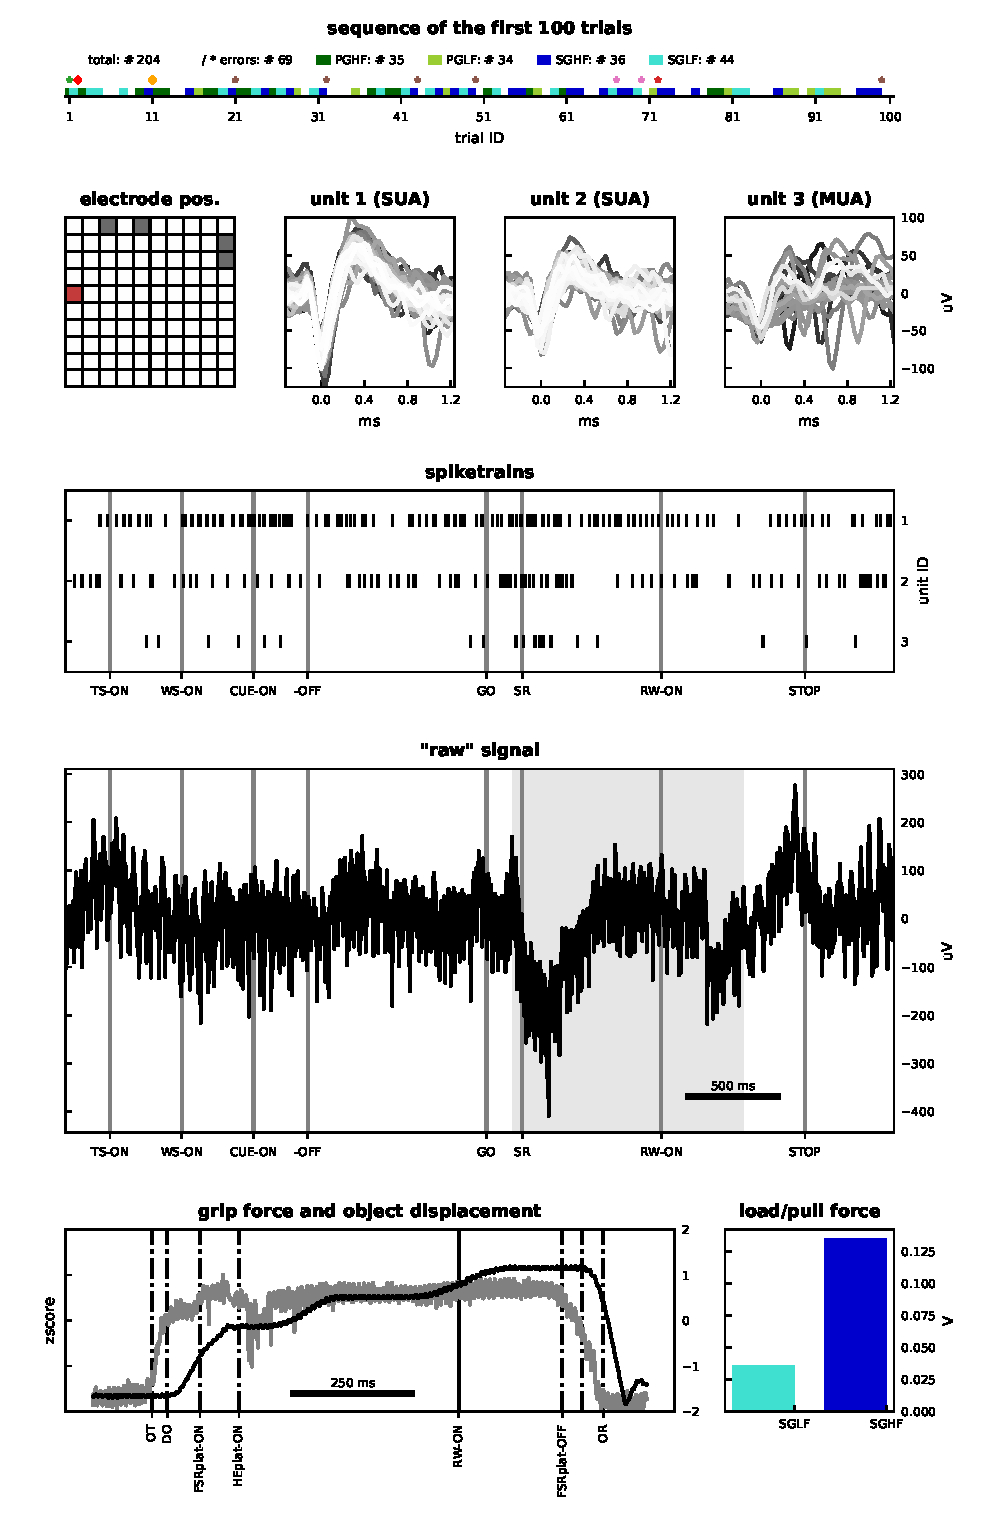
\includegraphics[width=\textwidth]{./figures/scidata_figures/data_overview_1_L}
 \caption[Overview of data types contained in l101210-001]{Overview of data types contained in l101210-001. The figure displays the different data types contained in the selected dataset of monkey L. Top panel: sequence of the first 100 trials (for trial types and errors see color in legend) and the total number of trials (see \# for correct, error, trial types in legend); the red diamond marks the selected trial (trial ID: 2) for panels below; the orange diamond marks an additional trial selected to demonstrate load/pull force differences between the averaged load force signals in the bottom right panel. Asterisks indicate error trials (black asterisks: grip errors). Second row, left panel: position of selected electrode (in red) for the data plots (electrode ID: 71). Second row, remaining panels: waveforms of three units from the selected electrode. Third row: spike trains of displayed units for the selected trial. Forth row: raw signal for the selected trial; gray shaded area marks the time window corresponding to the bottom left panel. Bottom left panel: grip force (gray) and object displacement (black) signals for the selected trial. Bottom right panel: averaged load/pull force signals for the duration of the plateau of the grip force signal for the selected LF and HF trial. Important trial events are indicated as vertical lines in the corresponding data plots.}
 \label{fig:overview_data_l_1}
\end{figure}

\begin{figure}
 \includegraphics[width=\textwidth]{./figures/scidata_figures/data_overview_2_L}
 \caption[Overview of raw signal and spike data of monkey L (l101210-001)]{Overview of raw signal and spike data of monkey L (l101210-001). Left panels: Raw signal (top) and spike data of unit IDs 1 on each given electrode (bottom) for a single trial (trial ID: 2) across a selection of electrodes. Right panels: Raw signal (top) and spike data from single unit ID 1 (bottom) across selected correctly performed trials on one electrode (electrode ID: 3). Trial events (TS-ON, WS-ON, CUE-ON, CUE-OFF, GO-ON, and RW-ON) are indicated as colored vertical lines in each plot. Trial types of selected trials in upper right panels are indicated as color (SGHF: dark blue; SGLF: cyan; PGHF: dark green; PGLF: light green)}
 \label{fig:overview_data_l_2}
\end{figure}

\begin{figure}
 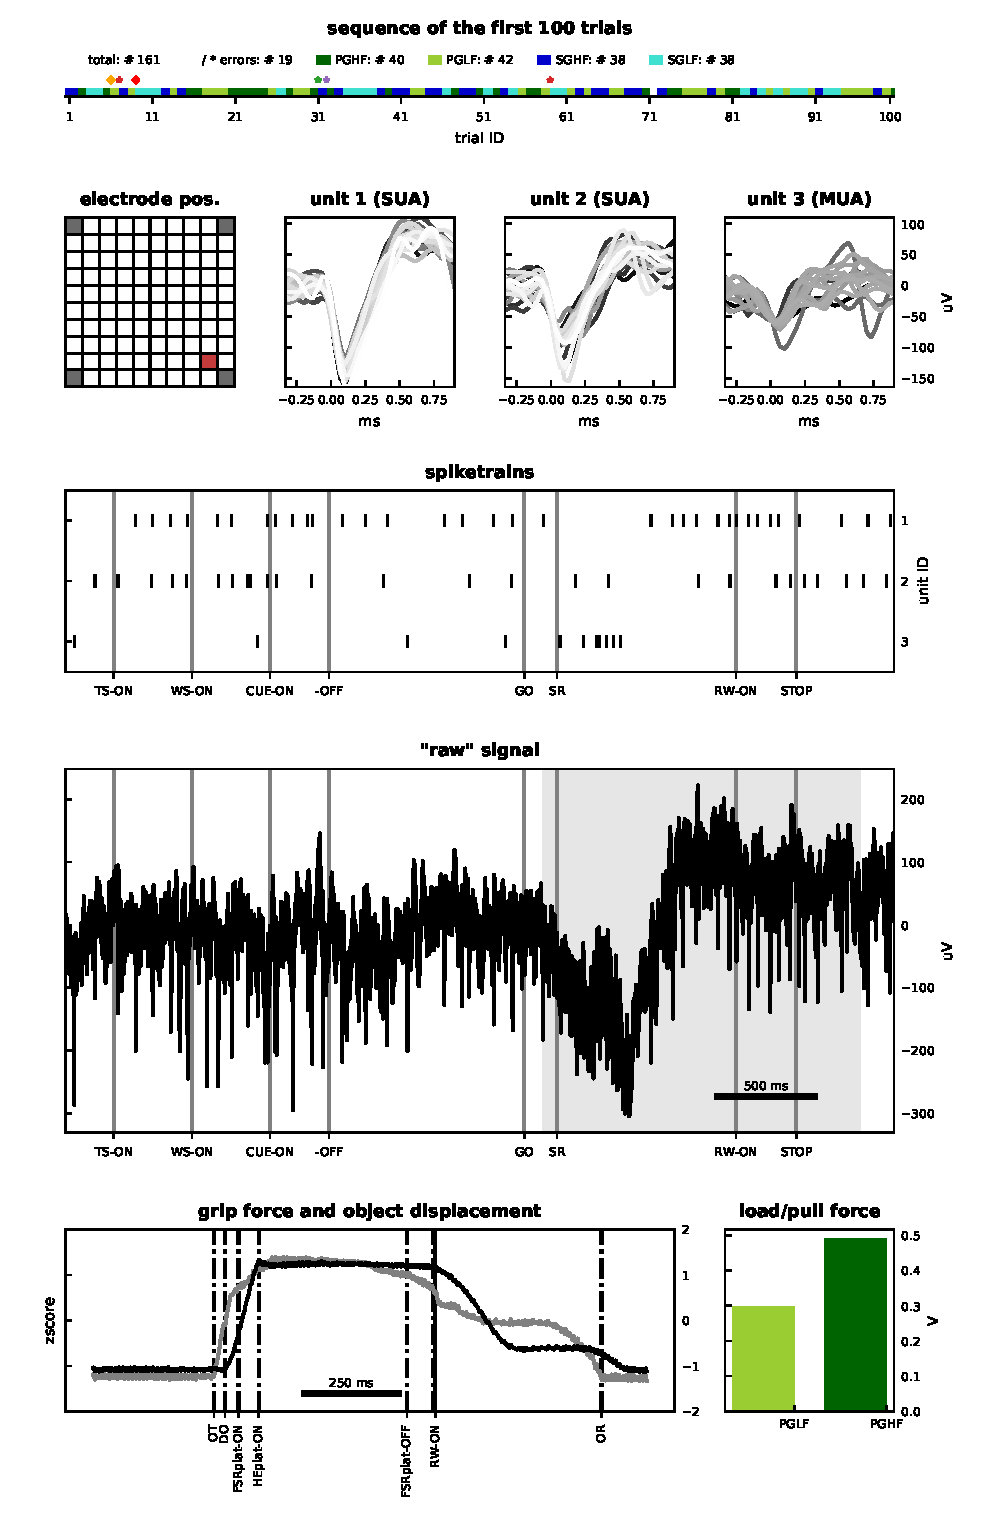
\includegraphics[width=\textwidth]{./figures/scidata_figures/data_overview_1_N}
 \caption[Overview of data types contained in i140703-001]{Overview of data types contained in i140703-001. The figure displays the different data types contained in the selected dataset of monkey N. Top panel: sequence of the first 100 trials (for trial types and errors see color in legend) and the total number of trials (see \# for correct, error, trial types in legend); the red diamond marks the selected trial (trial ID: 9) for panels below; the orange diamond marks an additional trial selected to demonstrate load/pull force differences between the averaged load force signals in the bottom right panel. Asterisks indicate error trials (black asterisks: grip errors). Second row, left panel: position of selected electrode (in red) for the data plots (electrode ID: 63). Second row, remaining panels: waveforms of three units from the selected electrode. Third row: spike trains of displayed units for the selected trial. Forth row panel: raw signal for the selected trial; gray shaded area marks the time window corresponding to the bottom left panel. Bottom left panel: grip force (gray) and object displacement (black) signals for the selected trial. Bottom right panel: averaged load/pull force signals for the duration of the plateau of the grip force signal for the selected LF and HF trial. Important trial events are indicated as vertical lines in the corresponding data plots.}
 \label{fig:overview_data_n_1}
\end{figure}

\begin{figure}
 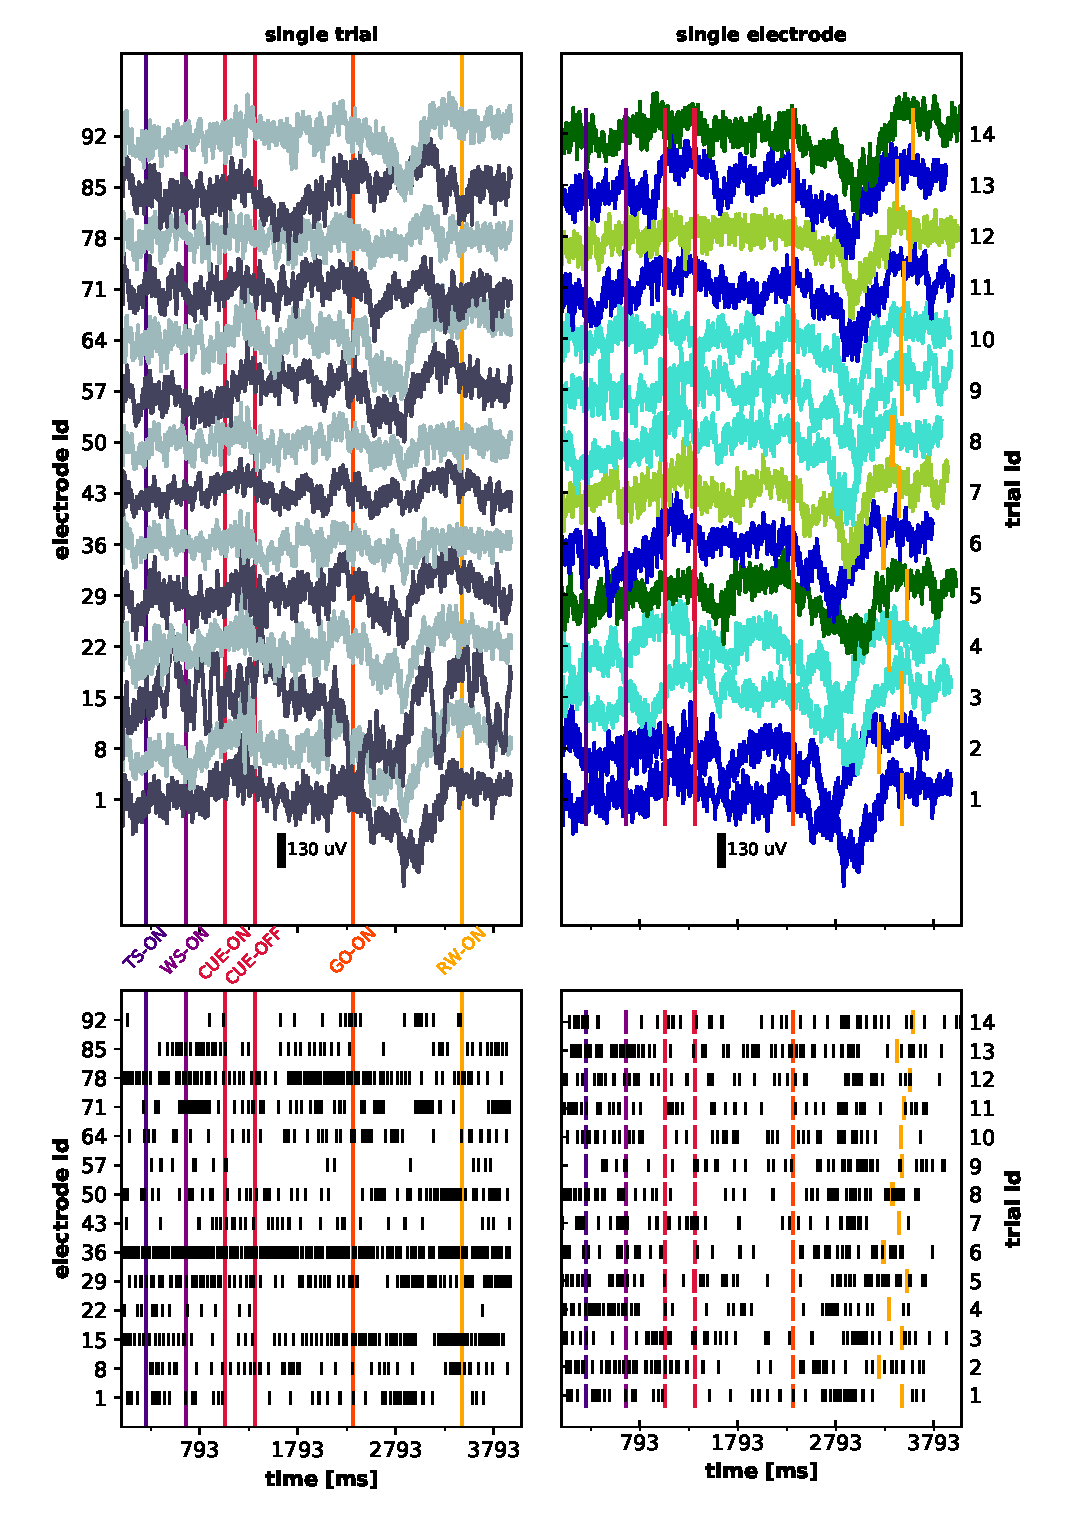
\includegraphics[width=\textwidth]{./figures/scidata_figures/data_overview_2_N}
 \caption[Overview of LFP and spike data of monkey N (i140703-001)]{Overview of LFP and spike data of monkey N (i140703-001). Left panels: LFP data (top) and spike data of unit IDs 1 on each given electrode (bottom) for a single trial (trial ID: 1) across a selection of electrodes. Right panels: LFP data (top) and spike data from single unit ID 1 (bottom) across selected correctly performed trials on one electrode (electrode ID: 1). Trial events (TS-ON, WS-ON,CUE-ON, CUE-OFF, GO-ON, and RW-ON) are indicated as colored vertical lines in each plot. Trial types of selected trials in upper right panels are indicated as color (SGHF: dark blue; SGLF: cyan; PGHF: dark green; PGLF: light green).}
 \label{fig:overview_data_n_2}
\end{figure}


Overview of recording days of the published datasets. For both monkeys, we chose to publish the first dataset (rec*-001) of the recording day. For details on the published datasets see \cref{tab:datafiles_trials} and \cref{tab:datafiles_overview}.

The dataset l101210-001 from monkey L is the first out of 9 recording sessions conducted on Friday, December 10, 2010, while the dataset i140703-001 from monkey N is the first out of only 3 recording sessions conducted on Thursday, July 3, 2014. Both datasets were recorded in the late morning. The following recording day went on for nearly one hour and a half for monkey L, and one hour for monkey N. Although the recording from monkey N lasted with 16:43 min several minutes longer than the recording from monkey L with only 11:49 min, monkey L executed 204 trials, while monkey N only performed 160 trials in total. However, monkey L performed only ~70\% of all trials correctly, whereas monkey N successfully completed ~90\% of all trials during the recording (cf. \cref{tab:datafiles_trials}). Nonetheless, the high percentage of error trials in monkey L are mainly caused by an too early movement onsets reflecting the eagerness, but also the nervousness of the monkey L's character. In contrast to these error types, monkey L used only 12 times the wrong grip compared to monkey N who performed an incorrect grip type 16 times during the recording. 

Overview of trials performed during the published datasets. Of the stated number of error trials, the monkey L and N used the wrong grip type in 12 and 16 trials, respectively. In the remaining error trials the monkeys initiated the movement too early. Trial types were altered randomly in the recordings which led to slightly different trial numbers for the different trial types.

For both monkeys the trial types alternated randomly between trials leading to slightly different numbers of trials with the same trial type in the each dataset (cf. \cref{tab:datafiles_trials}). 



The quality of the spiking activity in the datasets of both monkeys was high, which allowed us to perform a relatively robust offline spike sorting with high numbers of single unit activity (SUA) distributed over all electrodes of the array (for details see \ref{tab:datafiles_unitactivity}). For details on how the offline sorting was performed and checked please have a look at \cref{sec:offline_spike_sorting} and \cref{sec:spike_data_quality}. 
% 
% \begin{table}
% \begin{tabular}{|l|l|l|}
% \hline 
% \multicolumn{3}{|c|}{\textbf{monkey L}}\tabularnewline
% \hline 
% \textbf{file names} & \textbf{file size} & \textbf{file content}\tabularnewline
% \hline 
% \hline 
% l101210-001.ccf & 108.2 kB & cerebus configuration file\tabularnewline
% \hline 
% l101210-001.nev & 287.7 MB & digital events, unsorted spikes times \& waveforms\tabularnewline
% \hline 
% l101210-001-02.nev & 287.7 MB & digital events, sorted spikes times \& waveforms\tabularnewline
% \hline 
% l101210-001.ns2 & 8.5 MB & analog signals of object sensors\tabularnewline
% \hline 
% l101210-001.ns5 & 4.1 GB & raw neuronal signal\tabularnewline
% \hline 
% l101210-001.odml &  & metadata\tabularnewline
% \hline 
% l101210-001.mat &  & neuronal data annotated with metadata\tabularnewline
% \hline 
% \hline 
% \multicolumn{3}{|c|}{\textbf{monkey N}}\tabularnewline
% \hline 
% \textbf{file names} & \textbf{file size} & \textbf{file content}\tabularnewline
% \hline 
% \hline 
% i140703-001.ccf & 187.1 kB & cerebus configuration file\tabularnewline
% \hline 
% i140703-001.nev & 168.3 MB & digital events, unsorted spikes times \& waveforms\tabularnewline
% \hline 
% i140703-001-03.nev & 168.3 MB & digital events, sorted spikes times \& waveforms\tabularnewline
% \hline 
% i140703-001.ns2 & 204.7 MB & analog signals of object sensors and LFP signals\tabularnewline
% \hline 
% i140703-001.ns6 & 5.8 GB & raw neuronal signal\tabularnewline
% \hline 
% i140703-001.odml &  & metadata\tabularnewline
% \hline 
% i140703-001.mat &  & neuronal data annotated with metadata\tabularnewline
% \hline 
% \end{tabular}
% 
% \caption[Overview of files (names, size, and content) for each provided dataset of monkey L and N]{Overview of files (names, size, and content) for each provided dataset of monkey L and N. Besides the listed data and metadata files, we also provide a mat file collection from the dataset of each monkey that contains the analog and digital signals of the nev, ns5/6, and ns2 files annotated with the corresponding metadata information of the odml file.}
% \label{tab:datafiles_overview}
% \end{table}
% 
% \begin{table}
% \begin{tabular}{|c|c|c|c|c|c|c|}
% \hline 
% \multirow{2}{*}{\textbf{monkey}} & \multirow{2}{*}{\textbf{date}} & \multirow{2}{*}{\textbf{weekday}} & \multirow{2}{*}{\textbf{start}} & \multirow{2}{*}{\textbf{dur}} & \multirow{2}{*}{\textbf{\# rec}} & \multirow{2}{*}{\textbf{dur of rec{*}-001}}\tabularnewline
%  &  &  &  &  &  & \tabularnewline
% \hline 
% \hline 
% \textbf{L} & 2010-12-10 & Friday & 10:50 am & 01:28 h & 9 & 11:49 min\tabularnewline
% \hline 
% \textbf{N} & 2014-07-03 & Thursday & 10:41 am & 00:51 h & 3 & 16:43 min\tabularnewline
% \hline 
% \end{tabular}
% \caption[Overview of recording days of the published datasets]{Overview of recording days of the published datasets. For both monkeys, we chose to publish the first dataset (rec{*}-001) of the recording day. For details on the published datasets
% see \cref{tab:datafiles_trials} and \cref{tab:datafiles_overview}.}
% \label{tab:datasets_recday}
% \end{table}
% 
% \begin{table}
% \begin{tabular}{|c|c|c|c|c|c|c|c|c|}
% \hline 
% \multirow{2}{*}{\textbf{monkey}} & \textbf{\# trials} & \multicolumn{2}{c|}{\textbf{\# error trials}} & \multicolumn{5}{c|}{\textbf{\# correct trials }}\tabularnewline
% \cline{2-9} 
%  & 
% \textbf{total}
%  & 
% \textbf{total}
%  & 
% \textbf{grip}
%  & 
% \textbf{total}
%  & 
% \textbf{SG-LF}
%  & 
% \textbf{SG-HF}
%  & 
% \textbf{PG-LF}
%  & 
% \textbf{PG-HF}
% \tabularnewline
% \hline 
% \hline 
% \textbf{L} & 204 & 69 & 12 & 135 & 41 & 30 & 31 & 33\tabularnewline
% \hline 
% \textbf{N} & 160 & 19 & 16 & 141 & 35 & 35 & 35 & 36\tabularnewline
% \hline 
% \end{tabular}
% \caption[Overview of trials performed during the published datasets]{Overview of trials performed during the published datasets. Of the stated number of error trials, the monkey L and N used the wrong grip type in 12 and 16 trials, respectively. In the remaining error trials the monkeys initiated the movement too
% early. Trial types were altered randomly in the recordings which led to slightly different trial numbers for the different trial types.}
% \label{tab:datafiles_trials}
% \end{table}

\subsubsection{Information on metadata framework}
\label{sec:scidata_metadat_framework}

 All metadata information about the experiment, the subject, the setup, the settings, the processing of the data etc were originally distributed over several source files, but were collected offline in one metadata file per recording using the odML metadata framework. This odML framework was first introduced by \citet{Grewe_2011} and is a supported metadata management project of the G-Node (http://www.g-node.org/projects/odml). odML files are machine readable and can be used via application programming interfaces (APIs) in Java (https://github.com/G-Node/odml-java-lib), Python (https://github.com/G-Node/python-odml) and Matlab (https://github.com/G-Node/matlab-odml). Moreover, odML files are human readable and can be screened best by either using the odML Editor which is part of the odML Python API, or using a browser via a metadata stylesheet available as download on the G-Node project website. For details on how to manage metadata for such a complex experiment using the odML framework please have a look at \citet{Zehl_2016}. This reference also includes tutorial like code examples on how to use odML files in Python and Matlab (see main article as well as supplementary material).

\subsection{Technical Validation}

In addition to the above described preprocessing steps that needed to be performed to gain more content of the raw data, some technical validations of the data also had to be conducted. These technical validations include the correction of the irregular alignment data files of the Cerebus DAQ system and a general quality assessment of the data. In order to validate the quality of the recording, a series of algorithms were applied to the data. On the one hand the quality of the LFP signals was assessed per electrode and per trial by evaluating the variance of the corresponding signal in multiple frequency bands. On the other hand the quality of the offline sorted single units (\cref{sec:offline_spike_sorting}) was determined by a signal-to-noise measure. In addition, noise artifacts occurring simultaneously in the recorded spiking activity were detected and marked. In the following, we explain these technical validation steps in detail.

\subsubsection{Correction of data alignment}

The ns6 file starts always 82 samples later than ns5, ns2 and nev files. This miss-alignment is caused by an error in the Blackrock recording software. However, this shift is correctly recorded in the ns6 file, and therefore will be automatically corrected in the generic Neo loading routine (cf., BlackrockIO in \cref{sec:usage} below). In addition, due to the online filter procedure, the LFP signals in the ns2 file are delayed by approximately 3.6 ms with respect to the time stamps in the nev file and the analog signal of the ns6 file. This offset was heuristically determined, documented in the metadata file, and can be automatically corrected for by the experiment-specific loading routine (cf., ReachGraspIO in \cref{sec:usage} below). Note that the time stamps of the spike times provided in the nev file correspond to start of the waveform and not to the time point of threshold crossing.

\subsubsection{Quality assessment}

The occurrence of noise in electrophysiological recordings is to a certain degree unavoidable and therefore needs to be carefully examined. It depends to a large extent on the quality of the headstage used to record the neurophysiological data. In our data, two different types of headstages were used for the two monkeys - the Samtec-CerePort headstage (monkey L) and the Patient Cable (monkey N). The former is much more sensitive to noise than the latter. The type of noise, its cause and appearance in the data is quite variable. Depending on the direct influence of the different types of noise on subsequent analysis methods, one needs to balance the corresponding data rejection between being very permissive and very conservative. For this reason, it is wise not remove or delete data of bad quality, but instead mark them with the judgment of a corresponding quality assessment procedure. For the here published datasets, we provide the results of our quality assessment of the electrodes, trials and spiking units along with the analysis parameters of the used procedure in the odML metadata files for each recording. The reach-to-grasp IO integrates this information by annotating the corresponding data objects in Neo. This approach not only allows the user to finally decide which data to reject for an analysis, but also provides the opportunity to provide different quality assessments of the same electrode, trial and unit at the same time. This is helpful if one considers that certain types of noise can differently contaminate signals in different frequency bands. For the here published datasets, the quality of the recorded signals was therefore separately tested for the sorted spike data and different frequency bands of the LFP data. The used corresponding procedures are described in detail below. 

\subsubsection{LFP data quality}

The LFP data were examined for noise in three broad frequency bands excluding the 50Hz European line noise (low: 3Hz - 10Hz, middle: 12Hz - 40Hz, high: 60Hz - 250Hz) in each session individually. The goal of the quality assessment was, first, to detect channels with a noisy signal throughout the session and, second, to detect noisy trials in the remaining “clean” channels. To do so, the analog signals of each electrode were first z-scored and filtered in the three frequency bands (low, middle, and high) using a Butterworth filter (of order 2, 3, and 4, respectively). For each frequency band the quality assessment analysis was carried out separately. The detection of noisy electrodes was performed in three steps: 

step 1 The variance of the filtered analog signal of each electrode was calculated over the complete session. 

step 2 Out of the 96 resulting variance values, outliers were identified as those values outside a user-defined range. The range was defined as follows: (i) values between a lower (e.g., 25th) and an upper (e.g., 75th) percentile (L and U), (ii) the range of acceptable values was defined by $L-w\cdot(U-L),U+w\cdot(U-L)$,where w is a user-defined whisker coefficient (e.g., w=3). 

step 3 The analog signals classified as outliers in step 2 were visually controlled by comparing them to the analog signal of an electrode with a typical variance value. If the results were either too conservative or too permissive, the detection procedure was repeated by manually adapting the chosen parameters (L, U, and w), correspondingly. 

The electrode IDs of the final outliers as well as the parameters chosen for their detection were saved in the odML metadata file of the corresponding recording and marked as noisy for the tested frequency band. 

For the remaining non-noisy electrodes, an analogous procedure was carried out afterwards to detect noisy trials. The procedure differed in one respect: the variance of the filtered analog signal was calculated for each trial on each electrode separately. At the end, the trial IDs of the identified outliers were pooled and marked as noisy for the tested frequency band on all electrodes. The marked trial IDs were saved in the odML metadata file of the corresponding recording together with the chosen analysis parameters for their detection. Note again that with this procedure a trial is marked as noisy on all electrodes as soon as it is classified as noisy on one electrode.

\subsubsection{Spike data quality}
\label{sec:spike_data_quality}

To test and judge the quality of the spike data, the results of the offline spike sorting were controlled first, for the signal-to-noise ratio (SNR) from the waveforms of the identified single units and second, for the occurrence of hyper-synchronous event artifacts.

1. To calculate the SNR for each identified unit in the sorting results a method introduced by \cite{Hatsopoulos_2004} was used. The SNR was defined as the amplitude (A, trough-to-peak) of the mean waveform ($<w>$) divided by twice the standard deviation of the waveform noise ($SD_{noise}$) of the defined unit (u): $SNR_{u}=A_{<w>}/SD_{noise}\cdot2$,where $SD_{noise}$ was computed by averaging the standard deviations (SDs) obtained from each sample point across the original waveforms (SD of the waveform noise adapted from \cite{Nordhausen_1996,  Suner_2005}. For all identified single units in the datasets published here, the determined SNRs ranged between $1.5$ and $12$. Corresponding to \cite{Suner_2005} the quality of the spike sorting of an identified unit is good if the SNR is above 4, is fair if the SNR ranges between 2 and 4, and is poor if the SNR ranges between 1 and 2. Units with an SNR below 1 are not considered as signals. For a conservative analysis of the spike datasets, we recommend to use only single units with a SNR of 2.5 or higher, which was our choice in e.g. \cite{Torre_2016}. The results of the SNR analysis of the performed spike sorting were saved in the odML metadata file of the corresponding recording and units were annotated accordingly. 

2. \todo{Check with Emiliano(s papers). Synchrofact detection based only on SUA and not on all spikes?}Since correlation analysis of spike data is very sensitive to cross-electrode artifacts which would produce unwanted false positive results, we controlled the sorted spike data on their original time resolution ($\delta=1/30ms$) for potential occurrence of hyper-synchronous event artifacts. For this, we computed the population histogram, i.e. the sum of the spikes across all sorted single units in the dataset in bins of $\delta=1/30ms$ (sampling resolution of the data), and detected if there were entries $\ge2$. To our surprise these hyper-synchronous spikes, which are likely to be attributed to cross-channel noise, survived the spike sorting including the cross-channel artifact removal by the Plexon Spike sorter. We indeed detected these spike artifacts during a preliminary analysis of a previous study \cite{Torre_2016}. The number of single units participating in these events ranged from 2 to over 30 and a statistical analysis showed that the frequency of their occurrence largely exceeded the expected value considering the observed population firing rate. Furthermore, a $\delta$-binned time histogram of the population spiking activity triggered around the occurrence times of the hyper-synchronous events revealed also increased spiking activity in the preceding or following bin of the event. For a conservative analysis of the spike datasets, we recommend to treat the spikes participating in a hyper-synchronous event as well as the spikes occurring within a short time interval around this event ($\scriptstyle \pm\delta$) as artifacts of unknown origin and to remove them subsequently before performing any analysis of the spike data.

In \cite{Torre_2016} we combined both quality assessments of the spike data and only considered spikes with a SNR>2.5 and additionally removed all hyper-synchronous events with $\ge2$ spikes. 

\subsection{Usage Notes}
\label{sec:usage}

In the following, we describe how the provided data files can be practically used in a data analysis scenario. To this end, we first briefly present the open source software libraries we recommend to use in order to access data and metadata using the Python programming language. We also demonstrate how to merge data and metadata in a common representation that facilitates data handling and analysis. Finally, we present an example program that produces a visualization of the most important data items contained in the files, and can be used as a template script for accessing the provided data. All software discussed below is provided in the code subfolder of the provided datasets, and links to the code repositories are listed in \cref{sec:code_availability}.

As outlined above, the datasets are stored in two types of files. The primary data, and the spike sorted data, are provided in the data format (in particular, the nev, ns5 and ns6 format) specified by Blackrock Microsystems, the manufacturer of the recording hardware. Second, metadata are provided as one file in the odML format \cite{Grewe_2011}. While data and metadata are provided in documented file formats (see http://blackrockmicro.com/ and http://www.g-node.org/projects/odml, respectively), the mere knowledge of the highly complex internal structure of the files is insufficient to practically make use of their content. In particular, implementations of corresponding loading routines performed from scratch by individual researchers are likely to be incoherent and error-prone. Thus, in the following we will use two community supported open-source libraries to separately load primary data and metadata into a generic, well-defined data representation. 

We chose the data object model provided by the open-source Neo library \cite{Garcia_2014} as the primary representation of the datasets. Neo provides a hierarchical data structure composed of Python objects that aim to represent electrophysiological data in a generic manner. In addition, Neo provides a number I/Os that enable the user to read from (and in part, write to) a large number of open and vendor-specific file formats. In particular, Neo provides an I/O module for the file format used by Blackrock Microsystems (class BlackrockIO in file neo.io.blackrockio.py). The output of this I/O is a Neo data structure that is a faithful representation of the contents of the primary data files. For detailed information on the structure of the Neo data object model, please consult \cite{Garcia_2014} and the online documentation (http://neo.readthedocs.io/en/latest/index.html). The specific realization of the Neo output structure generated by the readblock() and readsegment() methods of the BlackrockIO are given in detail in the I/O's documentation. 

Here, we briefly summarize the output of the reach-to-grasp datasets obtained when calling the I/O. The readblock() method of an instantiation of the BlackrockIO returns a Neo Block object as a top level grouping object representing one recording session. In the hierarchy directly below the Block is one single Segment object spanning the complete continuous recording, and one ChannelIndex object for each of the 96 electrodes of the Utah Array (\ref{sec:surgery_array_location}) and each of the 6 sensor signals monitoring the target object manipulation (\cref{sec:experimental_apparatus}). The data from these 102 recording channels is each saved in one AnalogSignal object. All of these are linked to the Segment and the respective ChannelIndex object. Likewise, the spike times (and optionally, the spike waveforms) of each identified unit are saved to a SpikeTrain object. As for the AnalogSignal objects, these are linked to the Segment, and to the ChannelIndex object via a Unit object. Finally, all digital events are saved into a single Event object that lists their time of occurrences and the corresponding event IDs. Additional information from the file is provided as annotations on each individual Neo object (accessible via the annotation property of the object), in particular as annotations to the top level Block object. Note, that although this generic I/O can be used to access the raw data records, no interpretation of the file contents is given. For example, digital events are not interpreted as behavioral events, but only given as the raw numeric codes shown in \cref{fig:scidata_setup_overview}. 

In order to access the metadata stored in the odML file, we use the corresponding library API python-odML described in \cite{Grewe_2011}. In short, odML files store metadata in form of hierarchically structured key-value pairs. The odML files accompanying the provided datasets contain extensive metadata grouped into different sections describing different aspects of the experiment. A tutorial on how to work with the odML library can be found in the online documentation shipped with the library (https://g-node.github.io/python-odml/), and a more detailed description of how to manage metadata by example of the odML framework can be found in \cite{Zehl_2016}. In short, the library supports to read the content of an odML file, provides an API to navigate through the hierarchical structure, and to extract metadata of interest from the key-value pairs. Thus, the python-odML library provides a standardized way to access stored metadata records. 

As a next step, we combine the primary data and metadata in a manner that is specific to this experiment and aids the analysis process. To this end, the relevant metadata that were extracted from the odML are attached as annotations to data objects in the hierarchical Neo structure. For example, metadata information for a particular single unit originating from the spike sorting process may be attached to the Neo objects representing the sorted spike data of that unit. The task of combining the primary data and metadata is performed by a custom-written Python class named ReachGraspIO that is derived as child class from Neo's BlackrockIO class. For a full documentation of the input arguments, methods, and outputs of this class, please refer to the class documentation in reachgraspio.py. In short, invoking the readblock() method of the ReachGraspIO performs the following steps under the hood: (i) read the primary data using the readblock() method of the parent class (BlackrockIO) as described above, (ii) read the metadata using the python-odML library, (iii) interpret event data based on the digital events (e.g., detect trial start or reward), and (iv) add relevant metadata to the Neo data object using the annotation mechanism. Thus, the Neo Block object returned by the ReachGraspIO contains extensive information attached as annotations of the individual Neo objects, in particular, about whether a SpikeTrain is classified as SUA or MUA, about the spatial positioning of electrodes, or about the identities of electrodes that should be rejected. A full list of these metadata annotations can be found in the documentation of the readblock() method in the file reachgraspio.py.

In summary, for practical purposes, the resulting data structure of the ReachGraspIO hosts a complete representation of the data and a synthesis of the metadata relevant for analysis. This representation may be saved to disk in a standardized container format (e.g., .mat or HDF5), such that the exact same data and metadata context can also be accessed from other programming languages. For illustration, we provide the data object in the Matlab file format (.mat) in the folder datasets\_matlab, containing Matlab structs resembling the Python Neo objects.

In the following we demonstrate how to use the ReachGraspIO in practice in order to load and visualize the datasets. We follow the file example.py, which is contained as part of the code included with the published datasets. The goal of this program is to create a figure showing the raw signal, LFP, spikes (time stamps and waveforms), and events in a time window (referred to as analysis epoch) around TS-ON of trial 1 for electrode ID 62. 

In a first step, we load the data using the ReachGraspIO. Considering that only for monkey N an online filtered version of the LFP data is available in the ns2 file, in the following we calculate offline an LFP signal from all raw signals contained in the ns5 or ns6 files using a non-causal low-pass Butterworth filter implemented in the Electrophysiology Analysis Toolkit (Elephant; http://neuralensemble.org/elephant/), which provides analysis capabilities for data stored in the Neo representation. The parameters of this filter are chosen identical to those of the causal filter for the LFP recorded online in monkey N (\ref{sec:neural_recording_platform}).

In a subsequent step, we extract all TS-ON events in correctly performed trials. To this end, we use the function get\_events() contained in the utility module neo\_utils.py. The function extracts a list of events contained in one Event object of the loaded Neo Block given the filter criteria specified by the parameter event\_prop. In our example, the used filter criteria select all events from the Event object “TrialEvents” with a trial\_event\_labels annotation set to TS-ON, and a performance\_in\_trial annotation indicating a correct trial.

In a next step, we create Epoch objects representing analysis epochs around the extracted TS-ON events. To this end, we use add\_epochs() also contained in the utility module neo\_utils.py. The function excepts the previously extracted TS-ON events as trigger, and defines epochs of a given duration around this trigger. The resulting Epoch object is called “analysis\_epochs”. 

Next, we cut the data according to the analysis epochs and align the cutouts in time. This operation is performed by cut\_segment\_by\_epoch, which returns a list of Segment objects, each containing data of one analysis epoch. The Segments are annotated by the corresponding annotations of the Neo Epoch. In addition, the list of Segment objects is grouped in a new Neo Block, named “data\_cut\_to\_analysis\_epochs”. This representation now enables the analysis of the data across trials in the defined analysis epochs. 

In our example, we show how to create a plot of the data of the analysis epoch in one behavioral trial on the selected electrode. To select the Neo Segment corresponding to the first correct behavioral trial from the Block of the cut data obtained in the previous step, we apply the Neo filter() function. 

From the selected Segment, LFP data and raw signals can be obtained via the AnalogSignal objects referenced by the analogsignals property, while spike trains and corresponding unit waveforms can be extracted from the SpikeTrain objects referenced by the spiketrains property. The remainder of example.py uses the matplotlib library to create a figure of the data.

All data and metadata files as well as the code described above can be found in the data repository at \url{https://web.gin.g-node.org/INT/multielectrode_grasp}. The subdirectory datasets contains all data files and the metadata odML-file for the two provided recording sessions. The subdirectory code contains the files example.py and neo\_utils.py. For further reference and inspiration this subdirectory also contains the Python scripts generating the data figures of this manuscript. Furthermore, the subdirectories to code contain frozen versions of the required libraries (Neo, python-odml) as well as the custom loading routine combining data and metadata (reachgraspio.py). Finally, the datasets\_matlab directory contains the annotated Neo data object containing all primary data saved in the mat-file format. Updated versions of the code, e.g., adapted to new releases of the Neo library, can be found at https://github.com/INM-6/reach-to-grasp-data-publication.
}

\subsubsection{The metadata structure}
\label{sec:scidata_metadata_structure}
All aggregated metadata for a single recording session are collected in an separate \software{odML} file (\ref{tab:datafiles_overview}). Within an \software{odML} file, information is organized in a hierarchical fashion, following an experimenter-defined schema. \cref{fig:scidata_l101210odml} shows an exemplary part of the metadata collection of the recording session of monkey L. The \software{odML} files contains the following eight top-level sections: \textit{Project} (general information on the reach-to-grasp project), \textit{Subject} (information on the monkey), \textit{Setup} (details of the experimental apparatus), \textit{Cerebus} (settings of the recording system), \textit{UtahArray} (information on the multi-electrode array including spike sorting results and the corresponding quality assessment), \textit{Headstage} (general settings), \textit{Recording} (task settings, trial definitions with event time stamps and periods), \textit{PreProcessing} (results of LFP quality assessment and general information on the spike sorting procedure) (\cref{fig:scidata_l101210odml}). Each top-level \code{Section} contains a branch structure build from \code{Section}s to logically organize the information about the specific aspect of the experiment. For example, the \code{Subject} \code{Section} contains nine \code{Properties} (denoted by a folder icon), and two \code{Subsection}s, \code{Training} and \code{ArrayImplant} (denoted by a collapsible folder icon). All metadata available describing the training of monkey L are the coach (Thomas Brochier), start and end date of the training period (June 2010 - September 2010) and a comment stating that the training was easy and fast. Larger quantities of metadata are stored for describing the recording array used for the recording. Here the \code{Section} \code{UtahArray} contains general information about the hardware (material, dimensions, etc) and detailed information about each electrode is contained in the \code{Electrode} \code{Section}s. Each electrode \code{Section} contains information about the electrodes identity in different reference systems, the impedance value and offline sorting results for data recorded here (not shown in \cref{fig:scidata_l101210odml}). The metadata collection of monkey N has a analogous structure.

\begin{figure}
 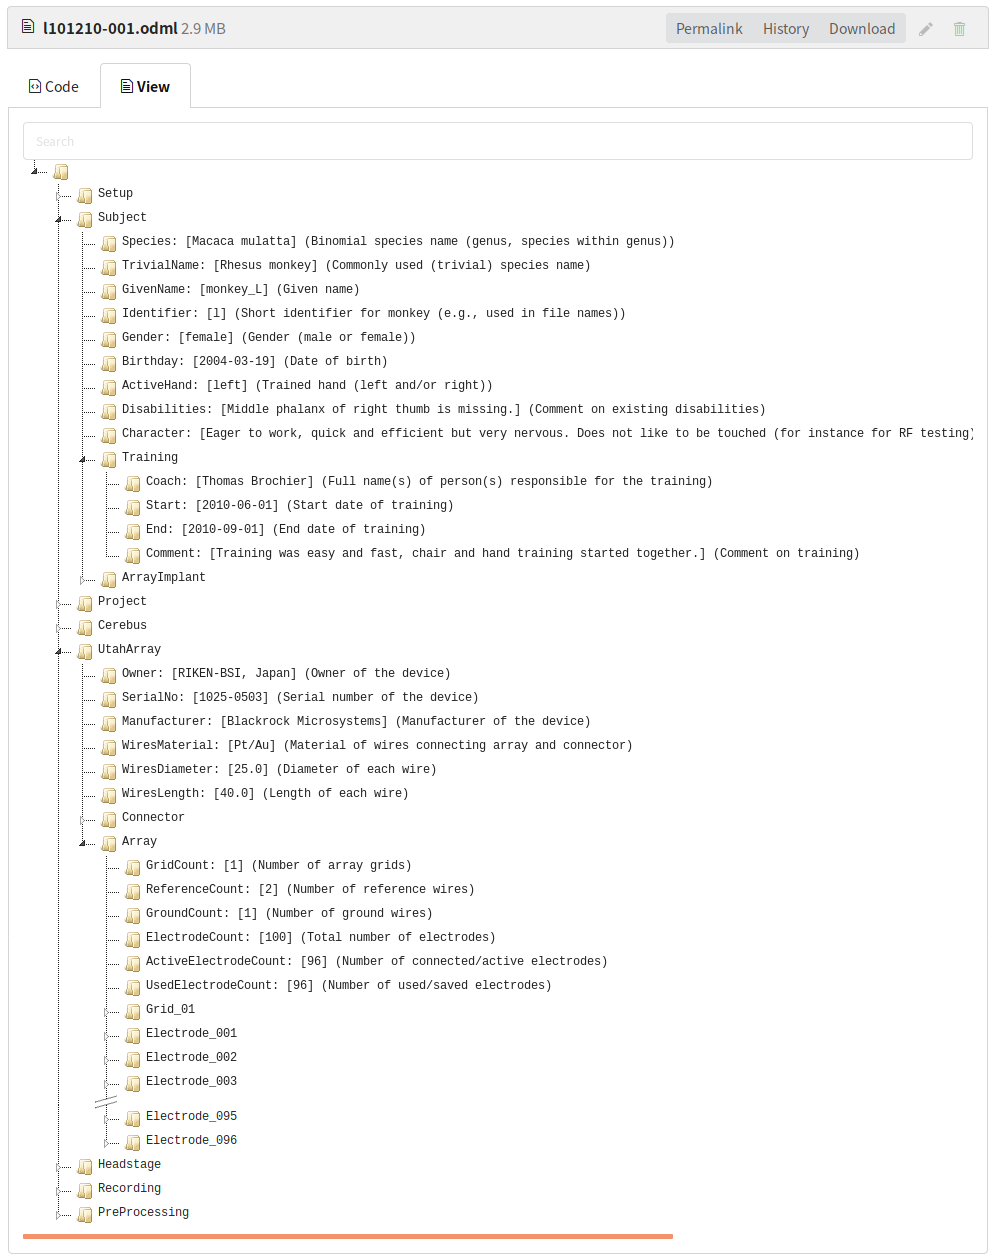
\includegraphics[width=\textwidth]{./figures/scidata_odmltree}
 \caption[Schematic metadata collection of session l101210-001]{Schematic metadata collection of recording session l101210-001 as rendered by the GIN webinterface. \code{Properties} are displayed in the form of \code{<Property Name>: <List of Values> (<Property Description>)}. Individual \code{Section}s are unfolded via user interaction to display the underlying metadata structure. Figure modified from \url{https://gin.g-node.org/INT/multielectrode_grasp/src/master/datasets/l101210-001.odml}.}
 \label{fig:scidata_l101210odml}
\end{figure}

\subsection{Preprocessing pipeline}
\label{sec:r2g_preprocessing_pipeline}
The metadata information as described \cref{sec:scidata_metadata_structure} was aggregated from multiple files and formats into a single file in the odML format (\cref{sec:scidata_metadat_framework}). This aggregation requires access to, and interpretation of a variety of files and formats, extraction of the corresponding information and integration in the designated location a pre-designed odML structure. In the pipeline used here (\cref{fig:scidata_metadata_pipeline}), the design of the odML structure is strictly separated from the enrichment of the structure with metadata content. In a first step an odML structure with default metadata entries is set up based on multiple Python scripts generating individual branches of the odML structure. Since the particular structure required for a recording session depends on the specifications of the recording this process depends to some extend on the metadata to be added (see \cref{fig:scidata_metadata_pipeline}, red arrows). This interdependency requires the metadata to be loaded and partially interpreted prior to the initialization of the structured metadata collection.

After construction of the odML structure metadata information is added via a number of custom enrichment functions. The enrichment is split into different functions, extracting information from the different specialized metadata source file formats and enriching the odML structure. In the enrichment process, the location of the target \code{Property} is implemented using a flexible approach exploiting the filter functionality of \software{odML}. This provides some degree of flexibility in handling the \software{odML} structure, but is computationally more intense then accessing the target location directly via its (in principal) know path. Finally, after building and enriching the metadata collection the \software{odML} file with more than $1300$ \code{Section}s, $8000$ \code{Properties} and about $10000$ \code{Value}s is saved.

Setting up this workflow required prepratory work on multiple levels: A) The manual preparation of the odML templates in dedicated Python scripts. These scripts mostly comprise more than 700 (maximum 1700) lines of code and contain the generation of all \software{odML} \code{Section}s and \code{Properties} including default \code{Value}s, since \code{odML} version 1.3 does not support empty \code{Values} of \code{Properties} (see \cref{sec:odml_model_revision}).  B) The preparation of the metadata source files in the required format. This involved \software{Plexon} supported manual offline spike sorting to generate a sorted \code{nev} file and spike sorting \code{mat} and text files containing the resulting metadata. For a single recording session this process requires a few working hours of a trained scientist. Additionally, xls sheets following the \software{odMLtables} standard needed to be set up containing information about the recording (sub)session, the monkey and the recording setup. Furthermore a single text file providing the mapping between different ID systems used in the experiment (\code{brain\_aligned\_elids.txt}) and the results of three \software{Matlab} based preprocessing scripts for detection of behavioural events based on continous signals (\code{even time markers} and \code{load detection}) and the quality checks for continous signals in multiple frequency ranges and electrodes (\code{rejections}) need to be provided. Most of these metadata source files are recording session specific and need to be generated after the recording was performed. Typically these files are generated by the experimenter at an \todo{arbitrary} time point after the recording \todo{up to years...}. C) The implementation of the odML generation pipeline (\cref{fig:scidata_metadata_pipeline} \code{odMLGenerator.py}) combining the \software{odML} structure from the templates with the content of the metadata sources. Implementation of this script needs detailed knowledge about both aspects of the \software{odML} generation process to be able to combine the two.

\begin{figure}
 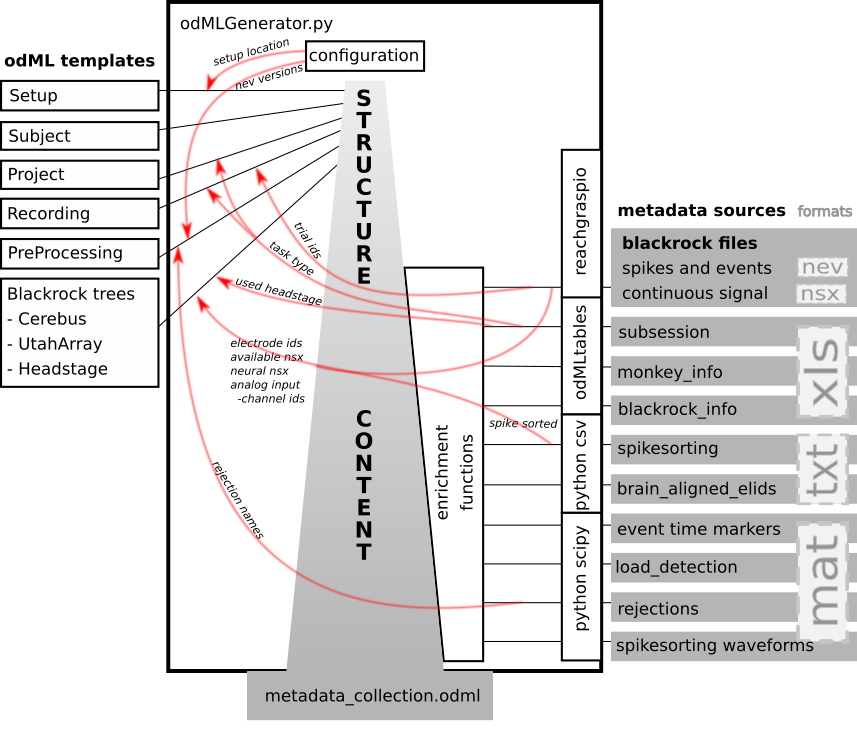
\includegraphics[width=\textwidth]{./figures/scidata_odMLgeneration_diagram}
 \caption[Schematic metadata aggregation pipeline used in \citet{Brochier_2018}]{Schematic metadata aggregation pipeline used in \citet{Brochier_2018}. The \software{odMLGenerator} script accesses \code{odML} templates and metadata source file in different formats. Based on a configuration file, first the structure of the \code{odML} is set up based on Python scripted \code{odML} templates. In a second step, the structure is enriched with information content from the metadata files. Information from these files is extracted using a variety of different tools (\code{reachgraspio}, \software{odMLtables}, the \software{Python} \software{csv} and \software{sicpy} packages) and added to the prebuilt \software{odML} structure via custom enrichment functions to generate the final metadata collection. Setting up the \software{odML} structure requires some information about the metadata (red arrows), which is extracted from the metadata files prior to the building of the \software{odML} structure.}
 \label{fig:scidata_metadata_pipeline}
\end{figure}

\subsection{Data loading and enrichment}
\label{sec:data_loading_and_enrichment}
To benefit from a complete metadata collection in the \software{odML} format when loading the original data we provide the \software{ReachGrapsIO} Python class which extends the \software{Neo} data structure upon loading (\cref{sec:usage}). The \software{ReachGraspIO} inherts from the \software{Neo} \code{BlackrockIO} and exploits its functionality to read data from \code{nsX}\footnote{$X \in \{1,2,3,4,5,6\}$} and \code{nev} file formats (\cref{fig:scidata_reachgraspio_diagram}). It returns a \software{Neo} \code{Block} based on the original structure generated by the \software{Neo} \code{BlackrockIO}. The API to interact with the data is therefore the same when using directly the \software{Neo} \code{BlackrockIO} and the \code{ReachGraspIO}.

The API of the \software{ReachGraspIO} is almost identical to the API of the \software{BlackrockIO}. The \software{ReachGraspIO} uses slightly different default parameters, which are adjusted to the datasets generated by the Reach-to-Grasp experiment. The usage of the \code{ReachGraspIO} is demonstrated in an example Python script, which loads the data and generates a minimalistic plot of the recorded signals at the time point of a trial start (\cref{code:scidata_visualization_1,code:scidata_visualization_2,fig:scidata_visualization}).
Identification and selection of a trial start event in the recording is facilitated by using the \code{ReachGrasIO} instead of the \code{BlackrockIO} as this identifies individual trials while loading the data and labels the trial events in a human readable fashion.


\begin{codeenv}
\inputminted[firstline=68, lastline=82, linenos,tabsize=2,breaklines, fontsize=\fontsize{7}{8}\selectfont]{python}{figures/scidata_figures/example.py}
\inputminted[firstline=86, lastline=86, linenos,tabsize=2,breaklines, fontsize=\fontsize{7}{8}\selectfont]{python}{figures/scidata_figures/example.py}
\inputminted[firstline=92, lastline=96, linenos,tabsize=2,breaklines, fontsize=\fontsize{7}{8}\selectfont]{python}{figures/scidata_figures/example.py}
\inputminted[firstline=99, lastline=119, linenos,tabsize=2,breaklines, fontsize=\fontsize{7}{8}\selectfont]{python}{figures/scidata_figures/example.py}
\inputminted[firstline=123, lastline=130, linenos,tabsize=2,breaklines, fontsize=\fontsize{7}{8}\selectfont]{python}{figures/scidata_figures/example.py}
\inputminted[firstline=143, lastline=148, linenos,tabsize=2,breaklines, fontsize=\fontsize{7}{8}\selectfont]{python}{figures/scidata_figures/example.py}
\inputminted[firstline=159, lastline=166, linenos,tabsize=2,breaklines, fontsize=\fontsize{7}{8}\selectfont]{python}{figures/scidata_figures/example.py}
\inputminted[firstline=174, lastline=176, linenos,tabsize=2,breaklines, fontsize=\fontsize{7}{8}\selectfont]{python}{figures/scidata_figures/example.py}
\caption[Example code for loading and processing of published data]{Example code for loading and processing of published data. Metadata annotated data is loaded (line 69-86) and a low pass filtered version of the original signals in generated (line 99-119). Trials are indentified and signals are cut into the corresponding segments (line 123-176).  Code extracted from \citet{Brochier_2018}, \url{https://gin.g-node.org/doi/multielectrode_grasp/src/master/code/example.py}}.
\label[codelisting]{code:scidata_visualization_1}
\end{codeenv}

\begin{codeenv}
\inputminted[firstline=195, lastline=253, linenos,tabsize=2,breaklines, fontsize=\fontsize{7}{8}\selectfont]{python}{figures/scidata_figures/example.py}
\caption[Continuation of \cref{code:scidata_visualization_1}: Plotting published data]{Continuation of \cref{code:scidata_visualization_1}. The plotting of the data belonging to the extracted trials for generation of \cref{scidata_visualization}. The figure is initialized and plotting parameters are defined (line 196-199). \code{AnalogSignals} are visualized (line 201-208) and \code{Spiketrains} are plotted together with the corresponding waveforms (line 213-230). \code{Event}s are visualized as vertical lines, labelled in human readable way (line 233-242). Finally, the plot is completed and saved in three different formats (line 244-153). Code extracted from \citet{Brochier_2018}, \url{https://gin.g-node.org/doi/multielectrode_grasp/src/master/code/example.py}}.
\label[codelisting]{code:scidata_visualization_2}
\end{codeenv}

\begin{figure}
 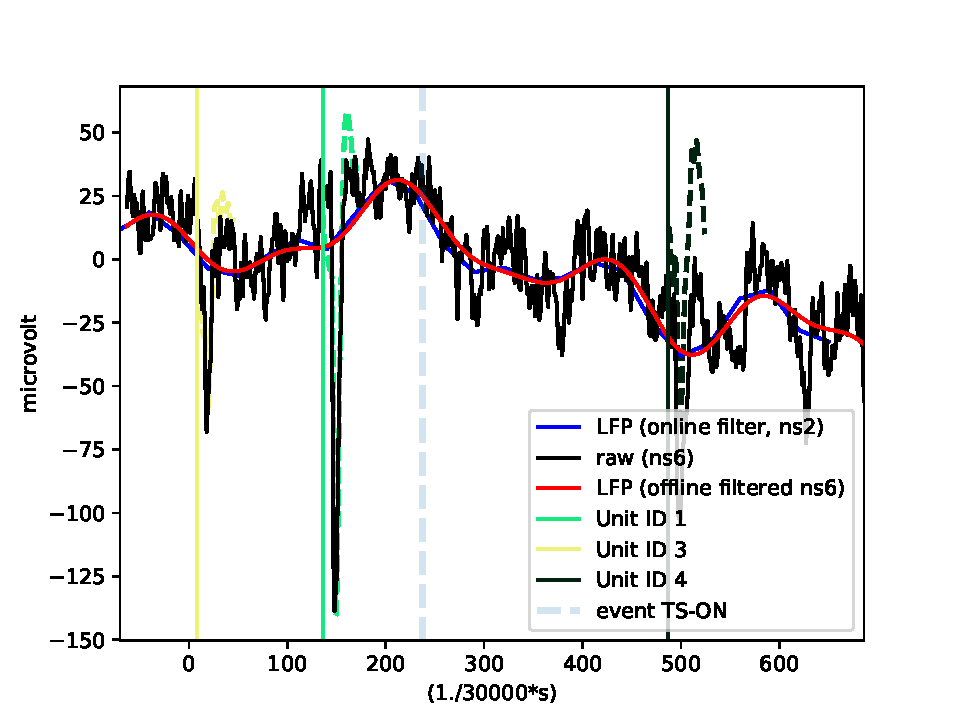
\includegraphics[width=\textwidth]{./figures/scidata_figures/example_plot}
 \caption[Example visualization of the published data]{Example visualization of the published data. The code to generate the figure is shown in \cref{code:scidata_visualization_1,code:scidata_visualization_2}. All recorded data from a single electrode are visualized: the raw, high resulution continous recording signal (ns6, black), the online filtered continous recording signal (ns2, blue) as well as an offline filtered version based on the raw signal (red). In addition spikes times are marked corresponing to their \software{Unit} assignment and online extracted waveforms are plotted (yellow, green and black traces). Trial events are also visualized (dashed vertical line) and labelled in human readable way (TS-ON, gray).}
 \label{fig:scidata_visualization}
\end{figure}

The \software{ReachGraspIO} extends and annotate the \software{Neo} structure generated by the \software{BlackrockIO} in multiple ways: continuous recording signals are corrected for time shifts introduced by online filters, event times extracted from analog signals are added and a merged representation of events from digital and analog sources is created (\cref{fig:scidata_reachgraspio_diagram}, red panels). The first two of these extensions depend on metadata being provided from the metadata collection in \software{odML} format. Additional annotations based on information from the metadata collection are added to most of the \software{Neo} objects (\cref{fig:scidata_reachgraspio_diagram}, gray panels). This includes basic metadata describing individual recording traces of \code{AnalogSignal}s, sorting information of \code{Unit}s, general metadata for \code{Segment}s and the \software{Neo} \code{Block} as well as information from the offline trial rejection. If no metadata collection is present, these extension and annotation steps are skipped. Some of these extension and annotation steps require also additional information, which is available within the \code{ReachGraspIO} as metadata lookup tables. These contain experiment specific code mappings which are essential for the interpretation of the data stored in the original \code{Blackrock} data files. This includes the mapping of bit-coded to human readable notation for events required to define a trial, event codes and equivalence groups, the mode in which the experiment is running (experimental conditions) as well as the performance codes standing for the outcome of a trial attempt (\cref{fig:scidata_reachgraspio_diagram}, green panels). These metadata lookup tables are used to translate the bit-based encoding of trial events into human readable versions. If an \code{odML} file is available, trial ids are extracted from there and also annotated. This interpretation of the events is a prerequisite for two further annotation steps: the identification of the task condition which again uses a \code{ReachGraspIO} lookup table, as well as the annotation of rejected trials. If digital and analog events are present, these will be merged in to a single \code{Event} object to simplify the access to all events of recording session (\cref{fig:scidata_reachgraspio_diagram}, 'merge digital \& analog events). Finally the \code{ReachGraspIO} returns the modified \software{Neo} \code{Block} which can be used in further data analysis and visualization scripts (e.g. see \ref{code:scidata_visualization_1,code:scidata_visualization_2}) or in the generation of a metadata collection (see \ref{fig:scidata_metadata_pipeline}).

\begin{figure}
 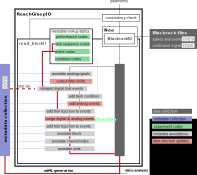
\includegraphics[width=\textwidth]{./figures/scidata_reachgraspio_diagram}
 \caption[Schematic data loading pipeline used in \citet{Brochier_2018}]{Schematic data loading pipeline used in \citet{Brochier_2018}. The \software{ReachGraspIO} utilized \software{Neo} to load the original recording data (top right). In a second step it enriches and extends the data structure based on additional metadata information from two sources: a metadata collection in \software{odML} format (blue) and ReachGraspIO internal lookup tables (green) containing the essential information required for interpretation the data from the original data files. The extension of the \software{Neo} structure includes correction of time shifts of the recording signals, addition of events which were offline extracted from analogsignals and the merging of multiple event arrays ('correct filter shifts', 'add analog events' and 'merge digital \& analog events', respectively; red panels). The enrichment of the \software{Neo} structure encompasses the addition of numerous annotations (gray panels). If no metadata collection is found, these steps are skipped. Finally the extended \software{Neo} structure is returned and can be used for the generation of a metadata collection or further processing and analysis steps. Dependencies contributing to a circular dependency of metadata are marked by bold arrows.}
 \label{fig:scidata_reachgraspio_diagram}
\end{figure}




The original pipeline was implemented using Python 2 and odML version 1.3. The published datasets were updated in 2019 to be compatible with Python 3 and odML version 1.4. Old versions are still accessible via the published DOI\footnote{10.12751/g-node.f83565, \url{https://gin.g-node.org/doi/multielectrode_grasp}} and the version control system of GIN\footnote{GIN, \url{https://web.gin.g-node.org/}}.

\subsection{Shortcomings of the odMLgeneration pipeline}
\label{sec:scidata_shortcomings}
% August 2019: 1974 datasets available at /datasets/marseille/congloue/data/DataGrasp
The presented data publication demonstrates the complexity of the datasets and the required preparation for release of the data. However, only two datasets out of almost 2000 recording sessions being performed were published due to multiple reasons:

% additional features in other datasets
\paragraph{Additional features}
\label{sec:additional_features_gaps}
The describing two datasets in a high degree of detail in a manuscript requires 23 pages of descriptor to provide all necessary details. Including additional datasets following the same experimental paradigm would expand the descriptor as additional features observed in the data need to be described. Extending the descriptor to include all peculiarities of all datasets will confound the reader therefore make the dataset less easily reusable.
An example for additional features which would require explicit description is an additional type of artifact, which is not described in \citet{Brochier_2018} as these two datasets do not exhibit unintended gaps during the recording. This type of artifact was first described in \citet{Sprenger_2014} and occurs when individual data packets are lost during data recording within the recording hardware. The loss of data packets does not cause in interruption of the recording or is tracked in the recording file, but the recording files appear intact. Lost data packets can only be detected afterwards by comparing raw continously recorded data with the corresponding online detected threshold crossing events. After the occurrence of a lost data packet, these two signal are not aligned, as only the continous signal is affected by lost data packages and not threshold crossing events.
\todo{Add a more detailed description of gappofacts? subsubsection?}

% thorough preparation of all preprocessing steps required
\paragraph{Manual validation}
Preparing the data for data publication requires implementation and cross check of all preprocessing steps (e.g. detection and correction of data packet loss) necessary for that particlar set of data. However, typically depending on the analysis aim, datasets are selected to be suited for the particular analysis, e.g. spiking activity from a session with lost data packets can still be used, as long as not compared to continously sampled data.  This typically means, that first only rudimentary preprocessing and artifact checking is performed on the datasets, and detailed, potentially manual checking of the data is only performed when required. 

% variability across datasets not covered by published version
\paragraph{Variability across datasets}
The pipeline for automatic metadata aggregation as presented here has been tested extensively for the two datasets published and the generated file have been manually checked. Running the exact same pipline on different recording datasets from the same recording is likely to fail, due to slight variations between recording sessions. A prime example for this is the set of event codes observed within a recording \ref{tab:bit_translation}. The observed event codes in this experiment highly depend on the monkey, as some react faster on provided cues, resulting in a specific event code being store and others react slower, wherefore the recording system already switched into another state and the action of the monkey is encoded differently.

% availability of source files
\paragraph{Availability of source files}
The preparation of source files for the metadata aggregation in to a single odML file is costly and requires thorough cross checking. Typically there is no dedicated person being responsible for this, but the task is shared between people being involved in the experiments. This results in a diffusion of responsibility, as all scientists also have additional projects to care about. For the discussed experiment, not all source file are available for all recording sessions, therefore the generation of an odML file will not succeed for part of the recording sessions. This mainly affects sessions, which are anyway not used for analysis due to other quality exclusion criteria.
\newline

In addition to the factors complicating the publication of numerous additional datasets from the same experiment as above, there are additional factors to be taken into account, when implementing a metadata aggregation pipeline of the complexity as presented here:

\paragraph{Multiple contributors}
In the case of multiple people being involved this also requires coordinated activity among all of them. Having individual copies of source files and running the metadata aggregation workflow using different configurations will lead to various, potentially inconsistent metadata collections. Also the updates of metadata need to be tracked and communicated in a reproducible manner.

\paragraph{Robustness \& Usability}
Special attention also needs to be invested making the execution of the pipeline (or minimally: the result of the exection) available to all collaborators, taking into account different needs and software (version) requirements of scientific projects. The pipeline therefore has to be robust to be run on different machines and different system environments and results need to be compatible with all analyis setups in use.

\paragraph{Structure \& Reusability} The presented metadata pipeline separates the structural templates of the odML and the enrichment with metadata values. This separation is a good approach during the design of the metadata workflow, as a general structure first needs to be established before implementing the enrichment. During the production phase of the odML generation however, this separation results in a coupling between the two phases, as for the enrichment of the \software{odML} structure knowledge about the structure is required. During the runtime of an experimental series frequently also adjustments and extensions need to be performed as the experimental design was updated or the need to track additional metadata was recognised. The modification and extension of the metadata structure during the production phase always require changes on both ends of the odML generation process, leading to an overly complex to adjust pipeline which is hard to maintain.

\paragraph{Linearity}
The presented pipeline for generating a metadata collection relies on the usage of the \code{ReachGraspIO} (\ref{sec:data_loading_and_enrichment}) for a basic interpretation of recorded events using the interal metadata lookup tables. Hard coding metadata in this manner is a reasonable approach to make the data quickly usable while the experiment is still under development, but in a stable configuration this introduces cyclic dependencies. In the example presented, the \code{ReachGraspIO} is relying on an (optional) \software{odML} file to provide metadata on the one side and on the other side the \software{odML} generation process depends on the usage of the \code{ReachGraspIO} (see \ref{fig:scidata_metadata_pipeline,fig:scidata_reachgraspio_diagram}). This introduces additional dependencies between software versions and metadata and convolutes the data loading from metadata interpretation and annotation aspect.

\paragraph{Portability} The presented metadata pipeline relies on specific versions of software packages, whereas the exact version required is not necessarily well documented. Running the workflow on different machines or moving the workflow to a high performance cluster requires expert knowledge and additional effort in setting up the correct environment for the workflow.

\paragraph{Consistency} Working with the published data requires multiple compatible files to be present: the original data files, the metadata collection, and multiple software packages. The version compatibility between all three aspects is typically only neglectfully documented and needlesly complicates the setup of a system to work with the data.



\subsection{Requirements for Maintainable and Reproducible Metadata Management}
\label{sec:metadata_requirements}
Based on the experience from publishing the two datasets (\ref{sec:scidata_shortcomings}) we identify essential requirements for metadata management workflows in complex, collaborative projects.

\begin{description}
 \item[R1: Common terminologies] To have a foundation of communication between collaboration partners it is important to agree on common terminologies. Within a scientific disciplin, this might be given by default, but as soon as scientists from multiple backgrounds need to interact, agreeing on common names is an essential first step. Concreting this in a documented way in the metadata collection is part of this and documents the terminology also for future generations of scientists.
 \item[R2: Structured machine \& human readable metadata] The metadata collection needs to be programmatically accessible to be used for data annotation and querying. However, metadata also needs to human readable, for manual checks and scanning of metadata. This becomes of special importance in the context of laboratory notebooks and how automatically generated metadata collections can substitute the manual notebooks in the long term. Finally, analysis results and figures need to be labelled in a human readable fashion for discussion and publication.
 \item[R3: Central data and metadata location] As discussed in \cref{sec:scidata_shortcomings}, in a collaborative environment a systematic organization of metadata is essential. Providing access to data and metadata via a central data storage is a straight forward solution. 
 \item[R4: Version control] To be able to communicate efficiently about data and metadata version control is an important tool. Using version control identical data and metadata selections by different scientist can be guaranteed on the one side as well as changes in the data and metadata collection can be tracked easily. This permits to track updates and changes on the data and metadata side and documents these in a basic manner.
 \item[R5: Mostly automatic metadata compilation] With the huge amount of metadata accumulating it is a high priority to automate metadata aggregation as far as possible. In some cases this is not possible in all cases, e.g. when metadata are only available in hand-written form in laboratory notebooks. This type of metadata however is a very small fraction of metadata and has in most cases to be digitized manually.
 \item[R6: Extendable metadata workflow] As discussed in \cref{sec:scidata_shortcomings} scientific metadata workflows need to be easily extendable to cope with latest analysis requirements and scientific findings.
 \item[R7: Reusability] Scientific workflows should be (partially) reusable for related projects to simplify the setup of similar workflows and save time in implementing these.
 \item[R8: Standardized \& reproducible preprocessing] Standardizing preprocessing steps improves understandability of the preprocessing tools and contributes to the aspect of reusability of the workflow. Making the individual preprocessing steps reproducible e.g. by provenance tracking used packages and documenting the code version helps making the whole workflow reproducible.
 \item[R9: Easy to access data and metadata for non-experts] Data and metadata should be easy to use by non-experts of the preprocessing pipeline. In the ideal case an out-of-the-box solution can be presented to the user, who can load the data immediately without installing a series of software dependencies. 
 \item[R10: Consistent data and metadata] Data and metadata should always be consistent, version control and reproducibility aid this.
 \item[R11: Open source tools] Open source software tools are transparent software packages which provide their source code to the community. This has the advantage of validation of the correct functionality by other users and permits to fix potential errors. For community software projects also code corrections and enhancements can be suggested and will usually be reviewed and integrated into the tool. Open source tools are free of charge and therefore provide a suitable basis for scientific work to be independent of industry.
\end{description}


\subsubsection{Evaluation of presented metadata pipeline}
\label{sec:r2gpipeline_evaluation}
The pipeline used for metadata aggregation and access in \citet{Brochier_2018} is described in \cref{sec:scidata_metadata_structure}. In \cref{sec:metadata_requirements} we identify a eleven requirements for comprehensive metadata management. In the following we evaluate the presented pipeline with respect to these requirements. \cref{tab:requirement_check_scidata} summarizes the findings.
\newline

The presented metadata pipeline consists of two main components: the \code{odMLGenerator} for integrating the metadata in a single \software{odML} metadata collection and the \code{ReachGraspIO} for data access and integration with metadata. By utilizing \software{odML} for metadata storage the requirement of having common terminologies (\requirement{R1}) is fulfilled in this pipeline, since \software{odML} requires the specification and definition of terms within the collection. This also guarantees that the metadata collection is machine and human readable (\requirement{R2}), as the \software{odML} is xml based and provides tools for user friendly visualization (odMLtables (\cref{sec:metadata}), odML-UI\footnote{\url{https://pypi.org/project/odML-UI/}}, odml\_view\footnote{\url{https://github.com/G-Node/python-odml/blob/master/odml/scripts/odml_view.py}}).

The pipeline itself does not include the automatic storage of data or metadata or related scripts at a central location (\requirement{R3}). However, combining the pipeline manually with a central server or a common data hosting platforms is easy as data as well as metadata files are self contained. By using a central data hosting platform which supports version control, like GitHub\footnote{\url{https://github.com/}}, GitLab\footnote{\url{https://about.gitlab.com/}} or GIN\footnote{\url{https://gin.g-node.org/}}, version control can be automatically introduced at the same time (\requirement{R4}). Alternative to using version control in combination with a remote server, a version control system can also be implemented locally, e.g. by using git\footnote{\url{https://git-scm.com/}}, git-annex\footnote{\url{https://git-annex.branchable.com/}} or git-lfs\footnote{\url{https://git-lfs.github.com/}} to version data locally.

The presented metadata pipeline is automated in the sense that it does not require direct manual interaction (\requirement{R5}). However, a fully automated workflow would include automatic initiation of the pipeline upon a change in the source files. This is not the case here, as there is no trigger mechanism included here. Possible extensions including this would be the integration of centrally hosted code in combination with a webhook to a continous integration service like Jenkins\footnote{\url{https://jenkins.io/}}, Travis\footnote{\url{https://travis-ci.org/}} or CircleCI\footnote{\url{https://circleci.com/}}.

The extendability (\requirement{R6}) of the presented workflow is limited, as changes in the metadata always require code changes in multiple places (see \ref{sec:scidata_shortcomings}, 'Additional features', 'Variability across datasets', 'Structure \& Reusability') and dependencies between structure and metadata need to be explicitly implemented in the \code{odML} generation process.

The separation between building the structure of the \software{odML} document and the enrichment with metadata makes parts of the structural templates usable for other experiments if they contain similar hardware, software or preprocessing components. However, the code for enriching these template structures is highly specific to the non-standardized formats of the metadata source files in this experiments. Therefore the reusability of the presented workflows for other exeperiments is limited to the structural template of the \software{odML} document (\requirement{R7}).

The compilation of the \software{odML} document in the presented pipeline is a single Python script relying on a number of additional Python packages for the aggregation process. No provenance is captured in the process and the final \software{odML} file does not contain any information about its genation process (\requirement{R8}). Possible extension to the workflow could be the usage of a provenance tracking tool like Sumatra\footnote{\url{https://pythonhosted.org/Sumatra/}} or explicit tracking of file and package versions used in the workflow.

For accessing the data in combination with the collected metadata in the \software{odML} format multiple software requirements need to be installed in specific versions: \software{Neo} for providing the data structure, \software{odML} for metadata handling, the experiment specific \code{ReachGraspIO} for combining the two as well as the original data files with a specific verison of the \software{odML} file. All of these have version interdependencies, which need to be considered when setting up an analysis based on the published data. Therefore installation of a analysis pipeline based on the published dataset requires some effort and time and can be demanding for non-experts (\requirement{R9}).

In the presented workflow the consistency of data and metadata is not explicitely checked. Especially after the \software{odML} file generation, there is no mechanism to validate the metadata and data (\requirement{R10}). An indirect mechanism to ensure consistency of data and metadata files is to introduce provenance tracking (\requirement{8}) in combination with version control mechanisms (requirement{R4}).

By using Python for the presented metadata pipeline in combination with the open-source software packages \software{odML}, \software{odMLtables} and \software{Neo} \citet{Brochier_2018} rely strongly on open-source software (\requirement{R11}). Some exceptions are preprocessing steps, which are required to generate the metadata source files, e.g. spike sorting using \software{Plexon} and a custom event detection implemented in \software{Matlab}. Also the recording setup is based on \software{Windows} and closed-source recording software by \code{Blackrock Microsystems}, but in priniple alternative open-source projects electrophysiology recordings (open ephys\footnote{\url{http://www.open-ephys.org/}} and spike sorting (e.g. tridesclous\footnote{\url{https://github.com/tridesclous/tridesclous}} exist, but need to be evaluated in the context of this and future projects.


\begin{table}[]
\begin{tabular}{|l|l|}
\hline
Requirement                                          &  \cite{Brochier_2018} \\  \hline
R1: Common terminologies                             &  yes \\ \hline
R2: Structured machine \& human readable metadata    &  yes \\ \hline
R3: Central data and metadata location               &  no \\ \hline
R4: Version control                                  &  no \\ \hline
R5: Mostly automatic metadata compilation            &  manual initialization \\ \hline
R6: Extendable metadata workflow                     &  minimal \\ \hline
R7: Reusability                                      &  partial \\ \hline
R8: Standardized \& reproducible preprocessing       &  no \\ \hline
R9: Easy to access data and metadata for non-experts &  partial \\ \hline
R10: Consistent data and metadata                    &  partial \\ \hline
R11: Open source tools                               &  mostly \\ \hline
\end{tabular}
\caption[Overview of workflow requirements for \cite{Brochier_2018}]{Overview of workflow requirements for \cite{Brochier_2018} based on requirements for data and metadata workflows as defined in \ref{sec:scidata_shortcomings}. The presented pipeline fullfills basic criteria regarding common terminilogy definition and structured and readable metadata and the usage of open source tools. Other criteria are partially or not met.}
\label{tab:requirement_check_scidata}
\end{table}



% \todo{
% shortcomings of the presented workflow
% - moderate reusability (due to template modularization, but not enrichment code)
% 
% general requirements for scientific workflow concepts:
% - versioning
% - reproducibility
% - 'out of the box' usability (user friendliness)
% - file size issues (with versioning (git/git-annex/gin \& loading of data)
% - central data hosting (especially for collaborative work)}
